\chapter{基于生成式对抗网络的图像编辑}

\section{引言}

生成式对抗网络~\cite{GANs}以一种对抗的方式训练生成器和鉴别器,从而对目标数据分布建模。当模型收敛时,生成器将从隐空间采样的隐变量映射到图像空间。最新的深度生成模型在生成逼真的图像方面取得了巨大进步,这些图像甚至与现实世界的照片无法区分。然而,GANs模型本身无法编辑生成图像的语义属性,比如操纵人像的年龄或场景图片的天气。

图像编辑可用于图像增强、动画设计等专业领域。目前基于GANs的图像编辑方法可以分为两类:图像空间编辑方法和隐空间编辑方法。图像空间编辑方法~\cite{cyclegan,i2i0,i2i1,i2i2} 将一张图像从源域直接转换到目标域。这些方法必须学习大量的冗余模型,因为每两个域之间的转换需要一个模型。这对于多属性编辑任务来说是灾难性的。
隐空间编辑方法侧重于在预训练的GANs的隐空间中搜索与语义相关的方向。这类方法按照监督信息可以进一步分为:无监督方法~\cite{icml2020,harkonen2020ganspace}、自监督方法~\cite{steer,variation} 和监督方法~\cite{interfacegan,iclr2021}。这类方法在做属性编辑时存在语义耦合的问题,改变一种属性通常伴随着其他属性的改变。语义耦合的根本原因在于,隐空间编辑方法所使用的预训练GANs在训练时没有受到属性的约束,其隐空间天然存在语义耦合。

为了从根本上解决这个问题,我们提出了一种输入属性与生成图像属性一致的生成式对抗网络,简称为属性一致的生成式对抗网络(Attribute Consistent Generative Adversarial Networks, ACGAN),用于图像属性编辑。
与现有方法不同,我们将隐空间分解为内容空间和属性空间:输入的隐变量由分别从内容空间(服从高斯分布)和属性空间(服从均匀分布)中采样的内容变量和属性变量组成。由于隐空间编辑方法发现的语义方向是耦合的,因此我们提出将属性空间投影到正交空间,以便将每个语义方向与其他方向分开。为了将可控语义方向投影到正交属性空间,我们进一步提出了一种属性一致损失,约束了生成图像的预测属性与输入属性变量之间的连续一致性。
然而,据我们所知,目前只有一个数据集Transient Attribute Database~\cite{scenedataset} 包含连续的属性标签,而大多数图像属性数据集~\cite{celeba,place,sun} 只包含二值标签。为了将我们的方法扩展到所有属性数据集,我们进一步提出了一种属性量化策略,将二值属性标签量化为连续值。

我们的属性一致性生成式对抗网络具有以下优点:
\begin{enumerate}
    \item \textbf{正交属性空间:} 将属性映射到预定义的正交空间。每个基向量在正交属性空间中的坐标表示属性强度。
    \item \textbf{属性一致性:} 生成图像的预测属性值与输入属性变量一致,有效将可控语义方向投影到正交属性空间。
    \item \textbf{连续属性量化:} 为了将我们的方法应用于更常见的二值属性数据集,我们计了一种属性量化策略来获得连续属性伪标签,可以灵活地与许多现有方法集成以提高编辑性能。
    \item \textbf{统一范式:} 在隐空间和生成模型中全面优化属性可控方向。通过增加可控参数来提高生成模型的属性敏感性。
\end{enumerate}

\section{属性一致性的生成式对抗网络}

\subsection{概述}
目前,大多数隐空间编辑方法都存在属性耦合的问题,因为它们不能保证发现的方向独立,这不可避免地导致隐空间中的语义耦合。为了从根本上解决属性耦合的问题,我们将生成器的隐变量分解为内容变量和属性变量,并将属性方向投影到正交空间中。
具体来说,我们提出了一种通过正交属性一致性进行图像编辑的属性一致生成式对抗网络(ACGAN),如图~\ref{fig:framework}所示。 在图~\ref{fig:framework}(a)中,方向搜索方法~\cite{icml2020, iclr2021}找到的方向是通过比较原始图像和编辑图像的属性差异来完成的,搜索到的方向互相耦合。图~\ref{fig:framework}(b)中我们的方法使用输入属性值和生成图像的预测属性之间的属性一致损失来训练生成器。 我们预定义的方向是正交的,以便将每个语义方向与其他方向分开。
这从根本上解决了隐空间编辑中的属性耦合问题,使同时编辑多种属性成为可能。

\begin{figure}
    \centering
    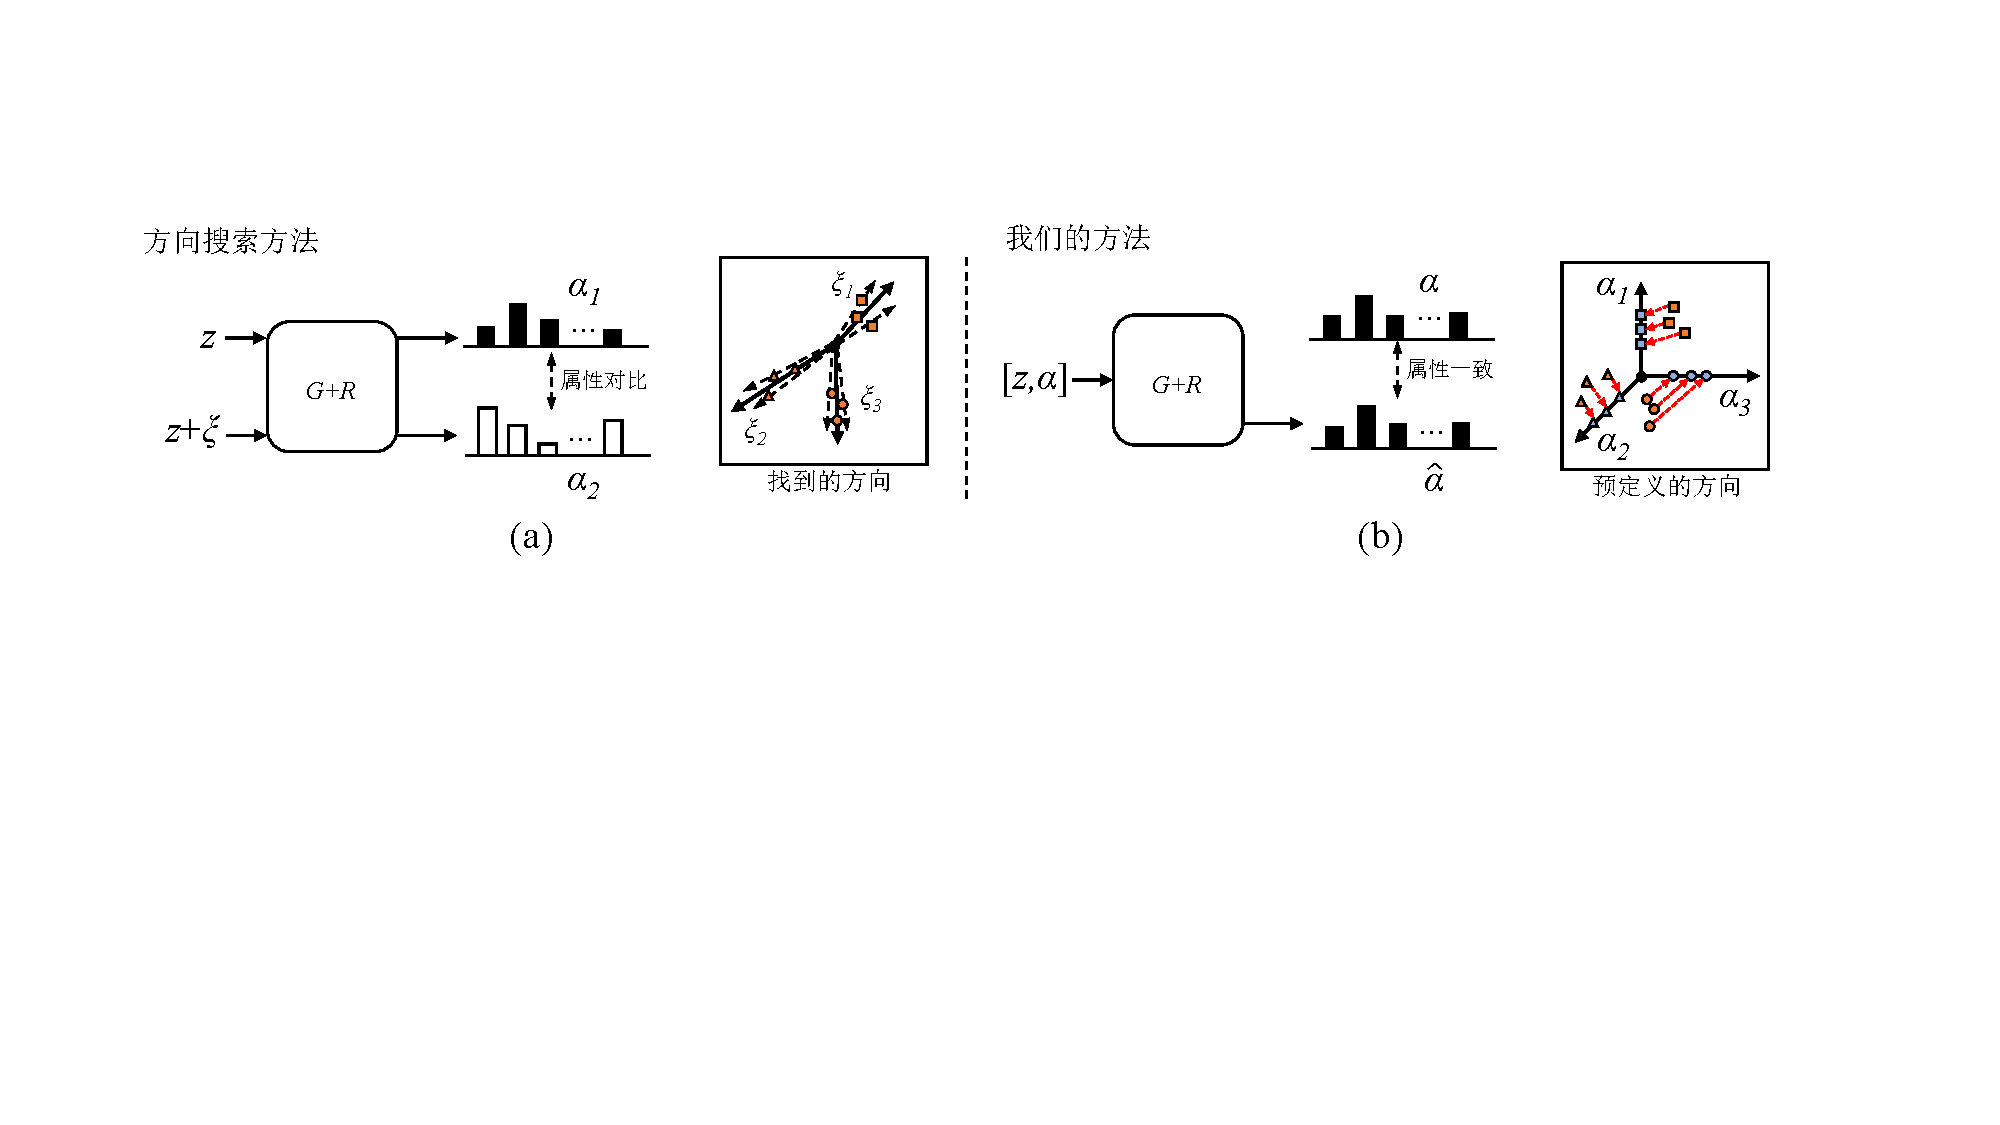
\includegraphics[width=1\linewidth]{figures/ACGAN/framework.pdf}
    \caption{方向搜索方法(左)和我们的方法(右)的框架}
    \label{fig:framework}
  \end{figure}

\subsection{连续属性标签量化}
% 形式化问题
% 对于给定的图片集$\{I_k\}_{k=1}^n \subset \mathbb{R}^{h \times w \times 3}$, 及其对应的属性集$\{y_k\}_{k=1}^n \subset \mathbb{R}^{d}$, 在这里$y_k$ is 0 for negtive or 1 for positive
假设我们有图片集 $\mathcal{D} = \{I_k\}_{k=1}^n \subset \mathbb{R}^{h \times w \times 3}$ 和属性集 $\mathcal{A} = \{y_k\}_{k=1}^n \subset \mathbb{R}^{d}$。 我们用 $\{I_k, y_k\}$ 表示数据集$\{\mathcal{D}, \mathcal{A}\}$种第 $k$ 张图片和其对应的属性标签。每个$y_k=[y_{k,1}, y_{k,2}, \cdot \cdot \cdot ,y_{k,N}]$, $y_{k,i}$的值是0或1, $N$是属性类别的数量。我们的目标是生成连续的伪标签 $\{\hat{y}_k\}_{k=1}^n$ 其中 $\{\hat{y}_k\}$ 包含 0 到 1 之间的连续值。

% 我们的想法是在$\mathcal{D}$上训练一个分类器,通过归一化分类器的置信度得到连续伪标签。
我们的想法是在$\{\mathcal{D}, \mathcal{A}\}$上训练一个由属性回归器$R_c$和一层$sigmoid$组成分类器,第$k$张图片分类置信度$x_{k}$的计算公式为:
\begin{equation}
     x_{k,i} = C(I_k) = sigmoid(R_c(I_k)),
\end{equation}
,分类器通过二值交叉熵损失训练:
\begin{equation}
     \mathcal{L}_{BCE} = \sum_{k=1}^n \sum_{i=1}^d [y_{k,i} \cdot \log x_{k,i}+\left(1-y_{k,i}\right) \cdot \log \left(1-x_{k,i}\right)],
\end{equation}
最后通过归一化分类器的置信度得到连续伪标签。

如图~\ref{fig:quantization}(b)所示,我们通过公式:
\begin{equation}
     \hat{y}_{k,i} = \frac{R_c(I_k)_i - \min \limits_{1 \leq t \leq n}R_c(I_t)_i}{\max \limits_{1 \leq t \leq n}R_c(I_t)_i - \min \limits_{1 \leq t \leq n}R_c(I_t)_i},
     \label{eq3}
\end{equation}
归一化 $\{R_c(I_K)\}_{k=1}^n$,生成了连续的属性标签。

注意这里的$R_c(\cdot)$不包含$sigmoid$运算。我们使用$sigmoid$运算之前的值,即$R_c(I_K)$,来计算量化属性值的原因在于$sigmoid$是一个“软”的阶跃函数:
\begin{equation}
   \chi_{A}(x)=\left\{\begin{array}{ll}
      0 & \text { if } x \leq 0 \\
      1 & \text { if } x > 0,
      \end{array}\right.
\end{equation}
$sigmoid$会将$R_c(I_k)$推至接近于0或1的值。

现在我们有了连续属性标签集$\hat{\mathcal{A}}=\{\hat{y}_k\}_{k=1}^n$。我们将在新数据集$\{\mathcal{D}, \hat{\mathcal{A}}\}$上训练新的属性回归器$R$,并将其用于监督生成器训练。


\begin{figure}[!t]
  \centering
  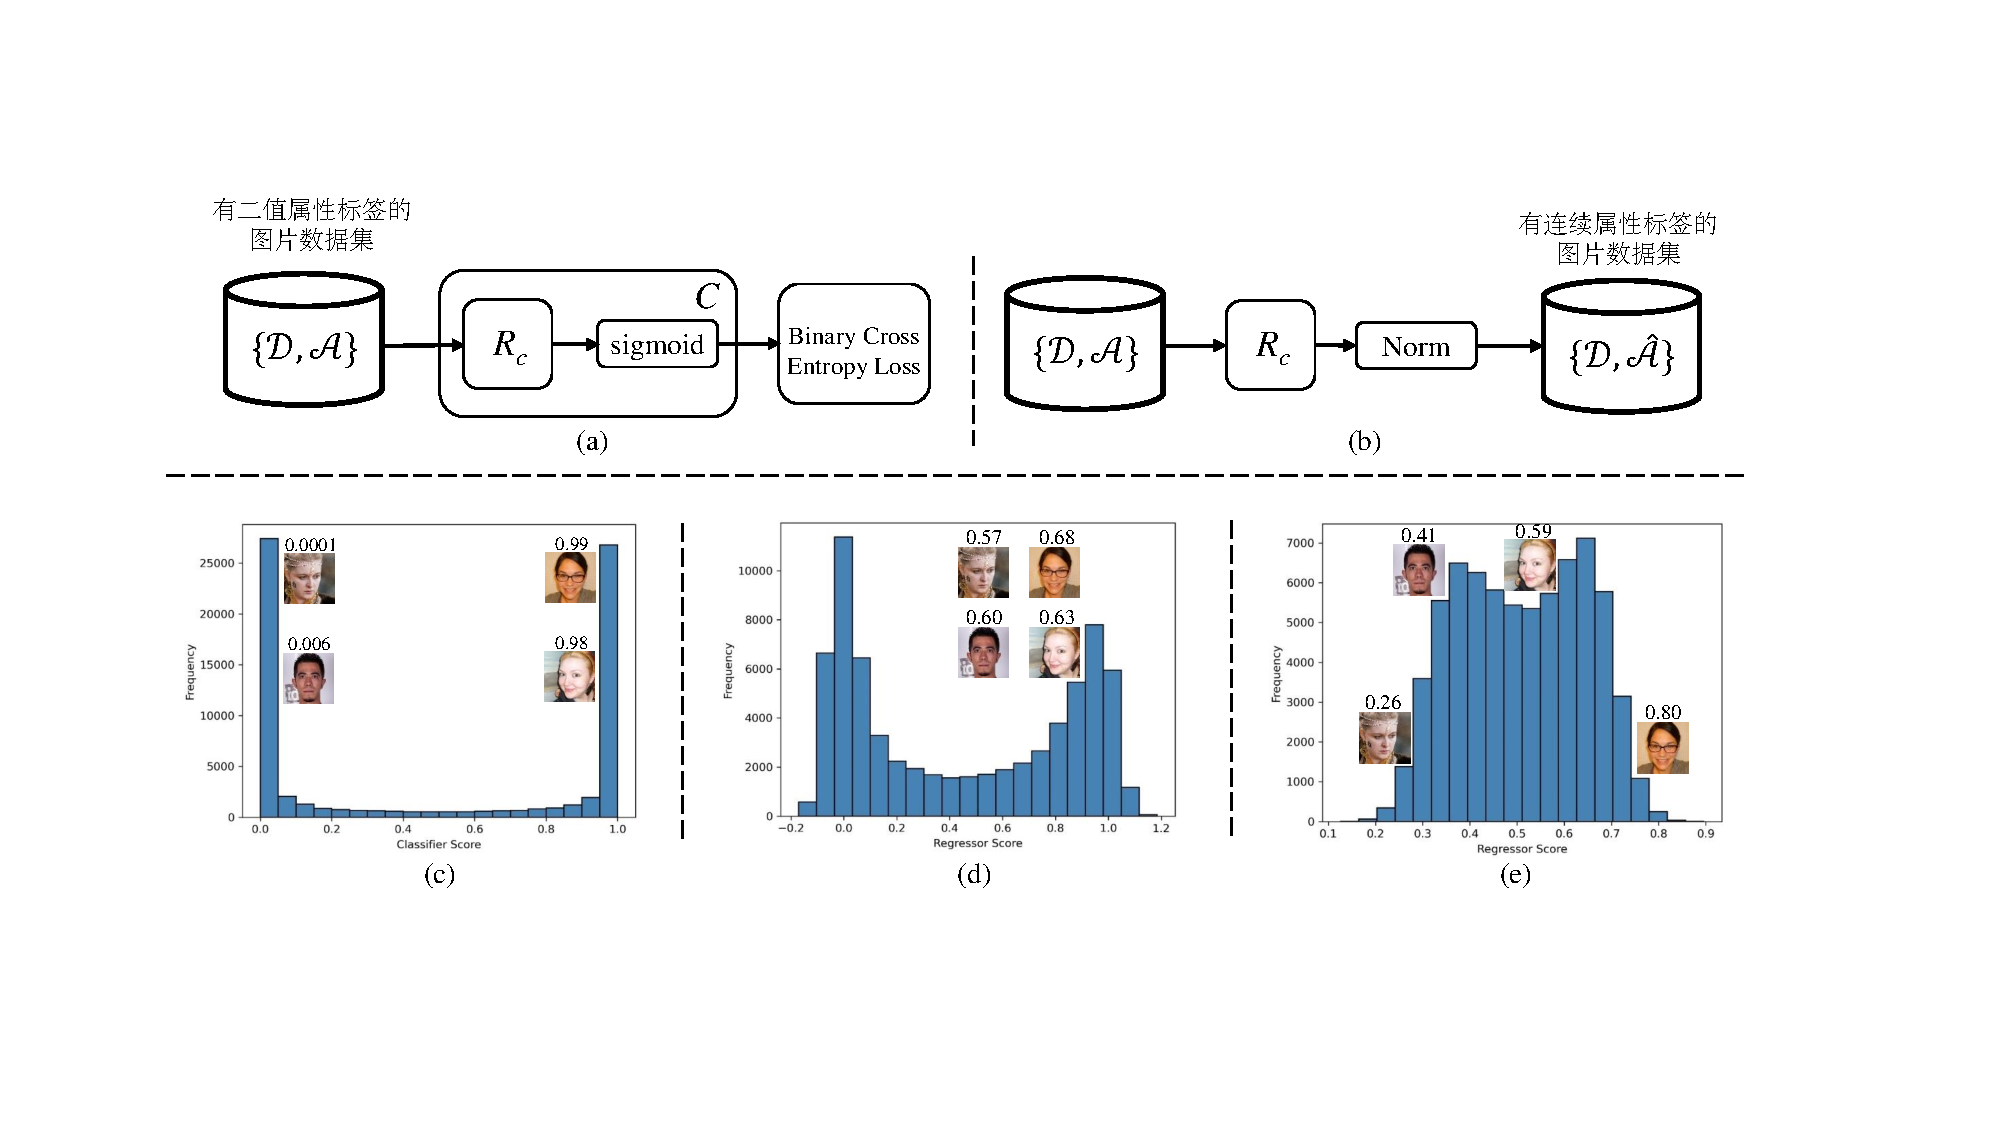
\includegraphics[width=1.0\linewidth]{figures/ACGAN/continue.pdf}
  % \caption{=连续属性生成。We first train an attribute classifier $C$ that consists of a continuous attribute regressor $R_c$ and a sigmoid layer as shown in (a) then we normalize outputs of $R_c$ as continuous labels as shown in (b). We collect attribute prediction values of classifier $C$ trained by $\mathcal{A}$, regressor $R_A$ trained by $\mathcal{A}$ and regressor $R$ trained by $\hat{\mathcal{A}}$ in (c), (d) and (e) respectively.}
  \caption{连续属性生成}
  % 我们首先训练属性分类器 $C$,它由一个连续属性回归器 $R_c$ 和一层 $sigmoid$ 组成,如(a)所示,然后我们将 $R_c$ 的输出归一化为连续标签,如(b)所示。 我们收集由 $\mathcal{A}$ 训练的分类器 $C$、$\mathcal{A}$ 训练的回归器 $R_A$ 和 $\hat{\mathcal{A}} 训练的回归器 $R$ 的属性预测值 $分别在(c)、(d)和(e)中。
  \label{fig:quantization}
\end{figure}

\subsection{属性一致性约束}
我们的ACGAN可以基于任意的非条件生成式对抗网络实现。ACGAN由3部分构成:生成器、判别器和属性回归器。我们将内容变量(高斯噪声,实现上相当于原来的隐变量)和属性变量共同作为网络的输入送入到生成器中,判别器的结构保持不变。属性回归器的作用是监督生成器的样本:生成器的训练目标不再仅仅是“骗过”判别器,还要满足生成样本的属性值与输入的属性变量一致。总之,在已有属性回归器的前提下,为了将任意的非条件生成式对抗网络改造成可以控制属性的ACGAN,仅需要做以下两点:1. 将生成器的输入扩充为隐变量和属性变量 2. 计算生成器的损失时加上属性一致性损失。
% \subsubsection{Overview} Our ACGAN can be implemented based on any unconditional GAN and is composed of 3 parts: a generator $G$, a discriminator $D$, and a pretrained attribute regressor $R$. Leaving the discriminator unchanged, the attribute code $\alpha$ and content code \emph{z} are fed into the generator as the inputs. $R$ is utilized to supervise the attributes of generated samples via attribute regression loss. The objective of the generator is no longer just to "deceive" the discriminator, but also to satisfy the attribute consistency, i.e., the attribute of the generated samples equal to the input attribute code. In short, in order to transform any unconditional GAN into ACGAN, only two changes need to be implemented: (1) decomposing the input values into content values and attribute values; (2) adding attribute regression loss.

\subsubsection{属性一致性损失}
ACGAN能够控制生成样本属性的关键之处在于在训练阶段生成样本的属性受到属性回归器的约束,这正是通过属性一致性损失(Attribute Consistency Loss)实现的。
% The key point to control the attributes of the generated samples is that the attributes of the generated samples are constrained by the attribute regressor in the training phase. This is achieved through minimizing $l_2$-norm between input attribute code $\alpha$ and predicted attribute $R(G(z|\alpha))$.% i.e., $\|R(G(z|\alpha)) - \alpha\|_2$.
% % \begin{equation}
% %      L_{Reg} =  \mathbb{E}_{z \sim \mathcal{N}(0,1), a \sim \mathcal{U}(0,1)}\|R(G(z|a)) - a\|_2
% % \end{equation}
% \begin{equation}
%      \|R(G(z|\alpha)) - \alpha\|_2
% \end{equation}

如何在训练阶段采样$\alpha$?我们在这里提供两种采样方式:1)从连续标签集$\hat{\mathcal{A}}$中采样 2)从均匀分布$\mathcal{U}(0,1)$采样。
当数据集中的属性在语义上存在耦合时,某些属性值的组合可能是不合理的。以CelebA数据集为例,山羊胡(goatee)和男性(male)这两种属性是高度耦合的,从常识上判断,男性为0但山羊胡的属性为1的组合是不合理的,
% How to sample $\alpha$ in the training phase? We investigate two sampling strategies: 1) sampling from the pseudo-label set $\hat{\mathcal{A}}$, 2) sampling from a uniform distribution $\mathcal{U}(0,1)$. 
% When attributes in $\mathcal{A}$ are semantically tangled, the combination of certain attribute values may be unreasonable. Taking CelebA dataset~\cite{celeba} as an example, the two attributes \textit{goatee} and \textit{male} are highly tangled. This combination is unreasonable where \textit{goatee} is 1 and \textit{male} is 0.

考虑到 $\hat{\mathcal{A}}$ 中的每个伪标签对应于 $\mathcal{D}$ 中的真实图像,第一种策略可以保证采样的 $\alpha$ 是合理的。
此时属性一致性损失可形式化为公式:
% Considering that each pseudo label in $\hat{\mathcal{A}}$ corresponds to a real image in $\mathcal{D}$, the first strategy can guarantee $\alpha$ is reasonable.
% Attribute-consistent loss can be formulated as:
\begin{equation}
   \mathcal{L}_{Reg}(G, R)  =  \mathbb{E}_{z \sim \mathcal{N}(0,1), \alpha \sim \hat{\mathcal{A}}}\|R(G(z|\alpha)) - \alpha\|_2
\end{equation}

至于第二种策略,我们可能会从 $\mathcal{U}(0,1)$ 中采样不合理的 $\alpha$,但是与第一种相比,这种采样策略有两个不可或缺的优势:

1) $\hat{\mathcal{A}}$ 中的属性值组合分布不均匀。让我们假设 $\alpha$ 中的每个变量都服从正态分布 $\mathcal{N}(0,1)$。如果我们直接从 $\hat{\mathcal{A}}$ 中采样 $\alpha$,中间属性值(接近 0.5)的采样概率最高,而采样极端属性值(接近 0 或 1)的概率) 会非常小。这实际上与我们的目标相矛盾:当输入属性从 0 线性变化到 1 时,我们希望 ACGAN 能够线性地生成相应属性值的样本。在这个过程中,我们平等对待中性属性值和极端属性值,因此从 $\mathcal{U}(0,1)$ 采样是一个更好的策略。

2) $\hat{\mathcal{A}}$ 中的样本可能有限。请注意,$\alpha$ 位于高维空间 $\mathbb{R}_N$ 中。当我们从 $\hat{\mathcal{A}}$ 中采样时,若假设${\mathcal{A}}$中共有$n$个样本,那么整个采样过程相当于在 $\mathbb{R}_N$ 中采样 $n$ 个点。如果我们采用第二种策略,采样点的数量取决于我们训练 ACGAN 的迭代次数,该次数远大于 n。
%As for the second strategy, we may sample unreasonable $\alpha$ from $\mathcal{U}(0,1)$, but this sampling strategy has two indispensable advantages compared to the first one: 

%1) Combination of attribute values in $\hat{\mathcal{A}}$ is quite biased. Let us assume that each variable in $\alpha$ obeys normal distribution $\mathcal{N}(0,1)$. If we directly sample $\alpha$ from $\hat{\mathcal{A}}$, the medium attribute value (close to 0.5) has the highest sampling probability, while the probability of sampling extreme attribute value (close to 0 or 1) will be very small. This actually contradicts our goal: when the input attribute changes linearly from 0 to 1, we wish ACGAN can linearly generate samples of the corresponding attribute value. In this process, we treat neutral attribute values and extreme attribute values equally, so sampling from $\mathcal{U}(0,1)$ is a better strategy.

%2) The samples in $\hat{\mathcal{A}}$ may be limited. Note that $\alpha$ lies in a high-dimensional space $\mathbb{R}_N$. It is insufficient to sample $n$ points in $\mathbb{R}_N$, but this is exactly what we do when sampling from $\hat{\mathcal{A}}$.If we adopt the second strategy, the number of sampled points depends on the number of iterations we train ACGAN, which is much larger than n.

一般情况下属性变量从均匀分布采样即可,此时属性一致性损失可以被形式化为:

% Generally, sampling $\alpha$ from $\mathcal{U}(0,1)$ is a more universal strategy. Attribute regression loss can be formulated as:
\begin{equation}
     \mathcal{L}_{cons}(G, R)  =  \mathbb{E}_{z \sim \mathcal{N}(0,1), \alpha \sim \mathcal{U}(0,1)}\|R(G(z|\alpha)) - \alpha\|_2
\end{equation}

% LGAN是
\subsubsection{网络总损失}
引入 $R$ 实现的属性一致性损失后,我们需要做的就是在原始 GAN 损失中加入属性回归损失:
% After introducing the attribute regression loss implemented by $R$, all we need to do is adding attribute regression loss to original GAN loss:
\begin{equation}
     \min _{G} \max _{D} V(D, G, R) = \mathcal{L}_{GAN}(G, D) + \lambda \mathcal{L}_{cons}(G, R),
     \label{overall}
\end{equation}
其中 $\mathcal{L}_{GAN}$ 是原始对抗损失,例如 WGAN~\cite{wgan} 中的 Wasserstein 损失或 LSGAN~\cite{lsgan} 中的最小二乘损失,$\lambda$ 是 $L_{cons}$的平衡超参数。
% where $\mathcal{L}_{GAN}$ is the original adversarial loss such as Wasserstein loss in WGAN~\cite{wgan} or least squares loss in LSGAN~\cite{lsgan}, $\lambda$ is a hyper parameter balancing $L_{Reg}$.

\subsubsection{ACGAN的训练算法}
我们在算法 ~\ref{al:acgan}描述了ACGAN的训练流程,可以看到与训练非条件GANs的最大区别在于训练过程中加入的属性一致性损失。

\begin{algorithm}[H]
\caption{ACGAN的训练算法}
\label{al:acgan}
\textbf{输入}: 预训练属性回归器 $R$, 生成器 $G$ 判别器 $D$, 批大小 $K$, 最大迭代次数 $M$, 图片数据集 $Q$, $G$的学习率$\mu_G$ 和 $D$的学习率 $\mu_D$\\
\textbf{参数}: $\theta_G$, $\theta_D$\\
\textbf{输出}: 判别器$D$和属性一致的生成器 $G$\\
\begin{algorithmic}[1] %[1] enables line numbers
\STATE 用参数 $\theta_G$ 初始化$G$,用参数 $\theta_D$ 初始化$D$,当前迭代次数$iteration=0$
\WHILE{$iteration \leq M$}
\STATE 采样 $z \sim \mathcal{N}(0,1), \alpha \sim \mathcal{U}(0,1)$;\\
    \STATE 生成 $I=G([z,\alpha])$;\\
    \STATE 计算 $\hat{\alpha} = R(I)$;\\
    \STATE 计算 $L=\mathcal{L}_{GAN}(G,D) +  \lambda \mathcal{L}_{Cons}(\alpha, \hat{\alpha})$;\\
    \STATE 更新 $\theta_G = \mu_G * \partial{L}/\partial{\theta_G}$;\\
    \STATE 更新 $\theta_D = \mu_D * \partial{L_{GAN}}/\partial{\theta_D}$;
\ENDWHILE
\STATE \textbf{return} $\theta_G$ and $\theta_D$
\end{algorithmic}
\end{algorithm}


\section{实验}

\subsection{实验细节}
我们在人脸合成和自然场景合成两个场景做了实验。 在本节中,我们将介绍 $C$ 和 $R$ 的基本模型和架构,然后分别描述这两个场景的实现细节。
% We conduct experiments on face synthesis and natural scene synthesis. In this section, we will introduce base model and architecture of $C$ and $R$, then describe implementation details in these two scenarios separately.

\subsubsection{基本模型} 
对于人脸合成场景,我们使用StyleGAN2~\cite{stylegan2} 实现了ACGAN;对于自然场景合成场景,我们则使用了轻量级 GAN~\cite{lwgan}。属性变量$\alpha$ 分别拼接在 轻量级 GAN 的 $z$ 和 StyleGAN2 的 $w$ 后面。
% We implement the proposed ACGAN based on light-weight GAN~\cite{lwgan} and StyleGAN2~\cite{stylegan2}. Due to the heavily computing cost of Stylegan2, we halve number of channels of convolution layer in each style block of Stylegan2. We term this more light weight Stylegan2 as Stylegan2-mini, which is adopted as the basic generative model  in the face synthesis experiments. The attribute code $\alpha$ is concatenated with $z$ for light-weight GAN and $w$ for StyleGAN2.

\subsubsection{$C$和$R$的结构}
我们采用 ResNet-50~\cite{resnet} 作为分类器 $C$ 和回归器 $R$ 的骨干网络,并且用维度为$N$的全连接层替换最后一个全连接层,这里的$N$为属性类别的数量,例如在CelebA数据集~\cite{celeba}数据集中$N=40$。 除$C$包含最后一层$sigmoid$外, $C$ 和 $R$ 共享相同的网络结构。 我们在 CelebA 数据集上训练分类器 $C$,达到 $96.05\%$ 的分类准确度。在 $\hat{\mathcal{A}}$ 上训练的回归器在验证集上的最小均方误差(MSE)达到 $0.0337$ ,在自然场景数据集~\cite{scenedataset} 上训练的回归器的MSE达到 $0.0142$。
% We adopt ResNet-50~\cite{resnet} as the backbone architecture of classifier $C$ and regressor $R$. The last fully connected layer is replaced by a new one with the dimension of $N$ corresponding to attribute categories. We isolate $sigmoid$ from attribute classifier $C$, so $C$ and $R$ can share the same network architecture. We train the classifier $C$ on CelebA dataset, which achieves $96.05\%$ of classification accuracy. The regressor trained on $\hat{\mathcal{A}}$ reaches validation MSE of $0.0337$ and the regressor trained on Transient Attribute Database~\cite{scenedataset} and reaches validation MSE of $0.0142$.

\subsubsection{数据集}
对于人脸合成,人脸属性知识是从 CelebA 数据集~\cite{celeba} 中学习的,这是一个大规模的人脸属性数据集,由超过 20万张名人照片组成。每张图像有 40 种属性标注,分辨率为 $178\times218$。 我们的 ACGAN 模型在 Flickr-Faces-HQ (FFHQ)~\cite{stylegan} 数据集上进行训练,该数据集由$70,000$的高质量图像组成,分辨率为$1024\times1024$,并且在年龄、种族和图像背景方面包含相当大的变化。 FFHQ训练的模型能够生成更真实的图像。
% For face synthesis, the facial attribute knowledge is learned from CelebA dataset~\cite{celeba}, which is a large-scale face attributes dataset consists of more than 200K celebrity images, each with 40 attribute annotations at $178\times218$ resolution. Our ACGAN model is optimized on Flickr-Faces-HQ (FFHQ)~\cite{stylegan} dataset, which consists of $70,000$ high-quality images at $1024\times1024$ resolution and contains considerable variation in terms of age, ethnicity and image background. FFHQ enables the model to generate high-fidelity images. 

% We select all 40 attributes for training as only a few attributes are mutually entangled.
对于自然场景合成,回归器 $R$在 Transient Attribute Database~\cite{scenedataset} 上训练。 由于该数据集具有介于 $0$ 和 $1$ 之间的连续属性值,因此没有必要训练属性分类器 $C$。 受EnjoyEditing~\cite{iclr2021}的启发,我们从Place数据集~\cite{place}和SUN数据集~\cite{sun}中选择了40,726张与自然场景相关的图片来扩展Transient Attribute数据集,并利用这个增强的自然场景数据集进行优化我们的ACGAN模型。
% For natural scene synthesis, the natural attribute knowledge is learned from Transient Attribute Database~\cite{scenedataset} for regressor $R$. Since this dataset has continuous attribute values between 0 and 1, it is unnecessary to train an attribute classifier $C$. Motivated by \cite{iclr2021}, we selected 40,726 pictures related to natural scenes from Place dataset~\cite{place} and SUN dataset~\cite{sun} to expand the Transient Attribute dataset, and utilized this augmented natural scene dataset to optimize our ACGAN model. 

% Unfortunately, lots of attributes are tangled, e.g., "daylight" and "night", "summer" and "winter". To avoid problem of tangled attributes discussed in Sec.\ref{section-31}, we select 5 attributes: "night", "clouds", "fog", "winter" and "sunny".

\subsubsection{其他实现细节}
我们设置超参数 $\lambda$ 来表示用于平衡属性回归损失的所选属性的数量,即人脸合成下$\lambda=40$,自然场景合成下$\lambda=5$。 $C$ 和 $R$ 均由 Adam 优化器训练,学习率为 0.0001。 我们使用单张 Titan RTX 进行所有实验。
% We set hyperparameter $\lambda$ to denote the number of selected attributes for balancing attribute regression loss, i.e., $\lambda=40$ for face synthesis and $\lambda=5$ for natural scene synthesis.  Both $C$ and $R$ are trained by an Adam optimizer with a learning rate of 0.0001. We use a single Titan RTX for all experiments.

\subsection{人脸属性编辑相关实验}
为了表示方便,我们统一使用+\{属性名\}表示增强该属性,相对应的,-\{属性名\}表示减弱该属性。

\subsubsection{定性比较}
在本节我们将定性评测单种属性和多种属性的编辑效果,并将我们的方法与两种有监督隐空间编辑方法进行比较:InterFaceGAN~\cite{interfacegan} 和 EnjoyEditing~\cite{iclr2021}。 截止文本撰写为止,EnjoyEditing的官方代码还没有发布,感谢他们简洁的框架,我们重新实现了他们的工作。为了公平地与这两种方法标胶,我们采用逆映射~\cite{image2stylegan}的方法将一张真实图像编码到 StyleGAN2 的隐空间中,以此比较同一图像上的属性编辑性能。
% We evaluate the attribute controllability on single and multiple attributes, and compare our method with two advanced supervised methods: InterFaceGAN~\cite{interfacegan} and EnjoyEditing~\cite{iclr2021}. Since the official code of EnjoyEditing is not released yet, we re-implement it by ourselves thanks to their concise framework. To fairly compare the performance of the two methods, we adopt \cite{image2stylegan} to encode one real image into the latent space of StyleGAN2, and compare the attribute editing performance on the same image.

图~\ref{fig:face} 显示了单属性编辑(b,c)和多属性编辑(d,e,f)的结果,Inversion表示逆映射方法得到的生成图像。 对于添加刘海,我们的 ACGAN 是唯一成功添加刘海的方法,而 InterFaceGAN 和 EnjoyEditing 只是将发际线向前移动了一点。 为了加胖,我们的 ACGAN 实现了最精确和最清晰的编辑结果。 InterFaceGAN的结果比原图要老,而EnjoyEditing的结果在增强胖属性方面不明显。
% Fig.~\ref{fig:face} shows results of single attribute editing (b, c) and multi attributes editing (d, e, f). For adding bangs, our ACGAN is the only method that adds bangs successfully, while InterFaceGAN and EnjoyEditing just move Hairline a little forward. For adding chubby, our ACGAN achieves most precised and distangled editing result. The result of InterFaceGAN is older than the original image, and the result of EnjoyEditing is not obvious at adding chubby.

对于多属性编辑评估,我们的 ACGAN 可以在不改变图像身份的情况下同时修改多种属性,如图~\ref{fig:face}所示。从编辑$1$种属性到$7$种属性,我们的ACGAN(第一行)展示出了非常精确的编辑效果。这$7$种属性包括:笑、肥胖、黑发、金发、口红、大鼻子 和 白皮肤。相比之下,基线无法添加某些属性或更改应保留的不相关属性。 InterfaceGAN 在图~\ref{fig:face}(c) 和 (d) 中涉及多属性编辑时对逆映射图像(Inversion)没有做太多改变。 当我们-棕头发时,EnjoyEditing 显然会将头发颜色变得更突出金色,纹理细节也变得更加模糊,从而导致人物整体外观更差,如图~\ref{fig:face}(d) 所示。
% For multiple attributes editing evaluation, our ACGAN can modify multiple attributes simultaneously without changing the image identity, as shown in Fig.~\ref{fig:face}. In contrast, the baselines fail to add certain attributes or change irrelevant attributes that should be preserved. InterfaceGAN does not make much changes to the inverted image when it comes to multiple attribute editing in Fig.~\ref{fig:face}(c) and (d). EnjoyEditing obviously changes hair color to be blonder when we decrease the \textit{blond hair} attribute. The texture details also become more blurred, which leads to a worse qualitative appearance as shown in Fig.~\ref{fig:face}(d).

\begin{figure}[!t]
     \begin{center}
        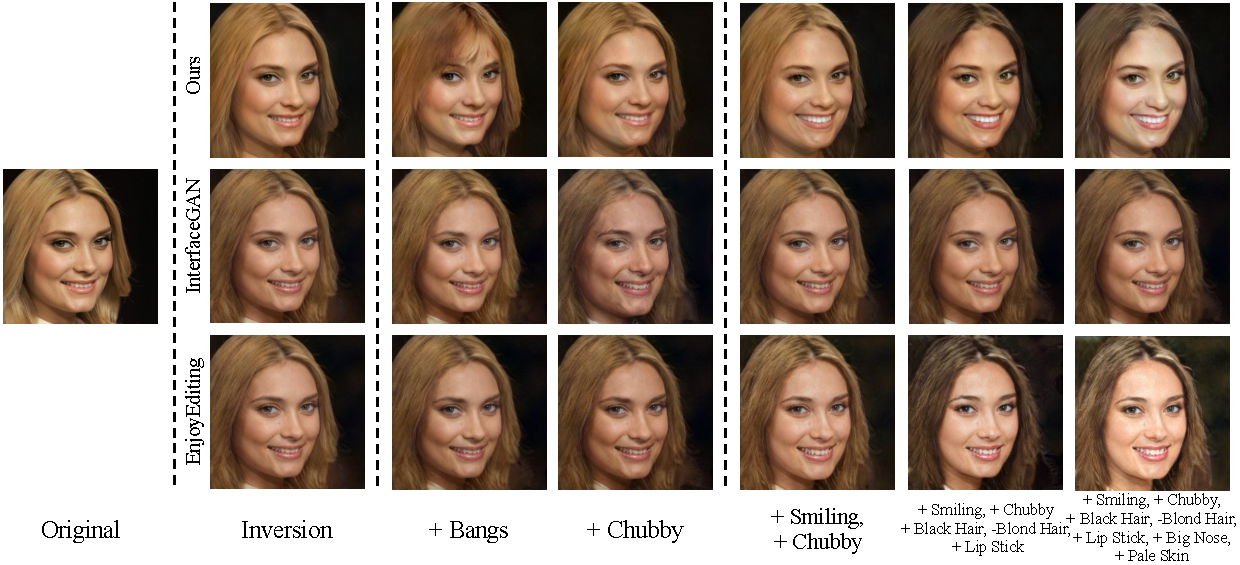
\includegraphics[width=1\linewidth]{figures/ACGAN/FaceMulti_center.pdf}
     \end{center}
     % \caption{Single attribute editing and multi attributes editing evaluation. On the first row, the results generated by our ACGAN are tremendously precise even for enhancing or reducing from $1$ to $7$ attributes including \textit{smiling, chubby, black Hair, blond Hair, lip stick, big Nose} and \textit{pale skin}. Please zoom-in for details.}
     \caption{单属性和多属性编辑的比较}
     \label{fig:face}
\end{figure}

\subsubsection{定量比较}
在本节我们提供两种定量方法,分别基于分类器评测与用户调研,来比较我们的方法与基准方法的性能差异。

为了评估属性编辑的准确性,我们统计了每种属性编辑的成功率和编辑一种属性时其他属性保持不变的的比例(我们称为保留率),这些指标均由预训练的分类器$C$计算得到。对于成功率,我们随机生成5000张图像并编辑所有这些图像的每种属性。我们的方法在所有属性中实现了 $84.13\%$ 的平均成功率,远高于 En​​joyEditing 的 $26.91\%$。在保留率的评估中,对于每种属性,我们收集5000张可以成功编辑该属性的图像,并统计其他未更改的属性比例。我们的方法实现了 $81.59\%$ 的平均保留率,这也优于EnjoyEditing。 图~\ref{fig:histogram} 具体比较了每种属性编辑的成功率和保留率。由于空间有限,并考虑到EnjoyEditing比InterfaceGAN的性能更好,我们只比较我们的方法和EnjoyEditing。我们的方法在大多数属性上的成功率和保留率达到了最高。
% To evaluate the attribute editing accuracy, we report the success rate of each attribute editing and the retention rate of irrelevant attributes while editing one attribute. These metrics are measured by a pretrained classifier. For success rate, we randomly sample $5,000$ images and edit each attribute for all these images. Our method achieves $84.13\%$ of averaged success rate among all the attributes, which is much higher than $26.91\%$ of EnjoyEditing. In the evaluation of retention rate, for each attribute, we generate $5,000$ images that can successfully edit this attribute and measure the other unchanged attributes. Our method achieves $81.59\%$ of averaged retention rate, which is also superior than EnjoyEditing. Fig.~\ref{fig:histogram} presents the comparisons on each attribute. Our method achieves the superiority performance on all the attributes for success rate and advanced accuracy on most attributes for retention rate. We also provide multiple attribute editing comparisons in the supplementary material.

% 柱状图
\begin{figure}[!t]
    \begin{center}
         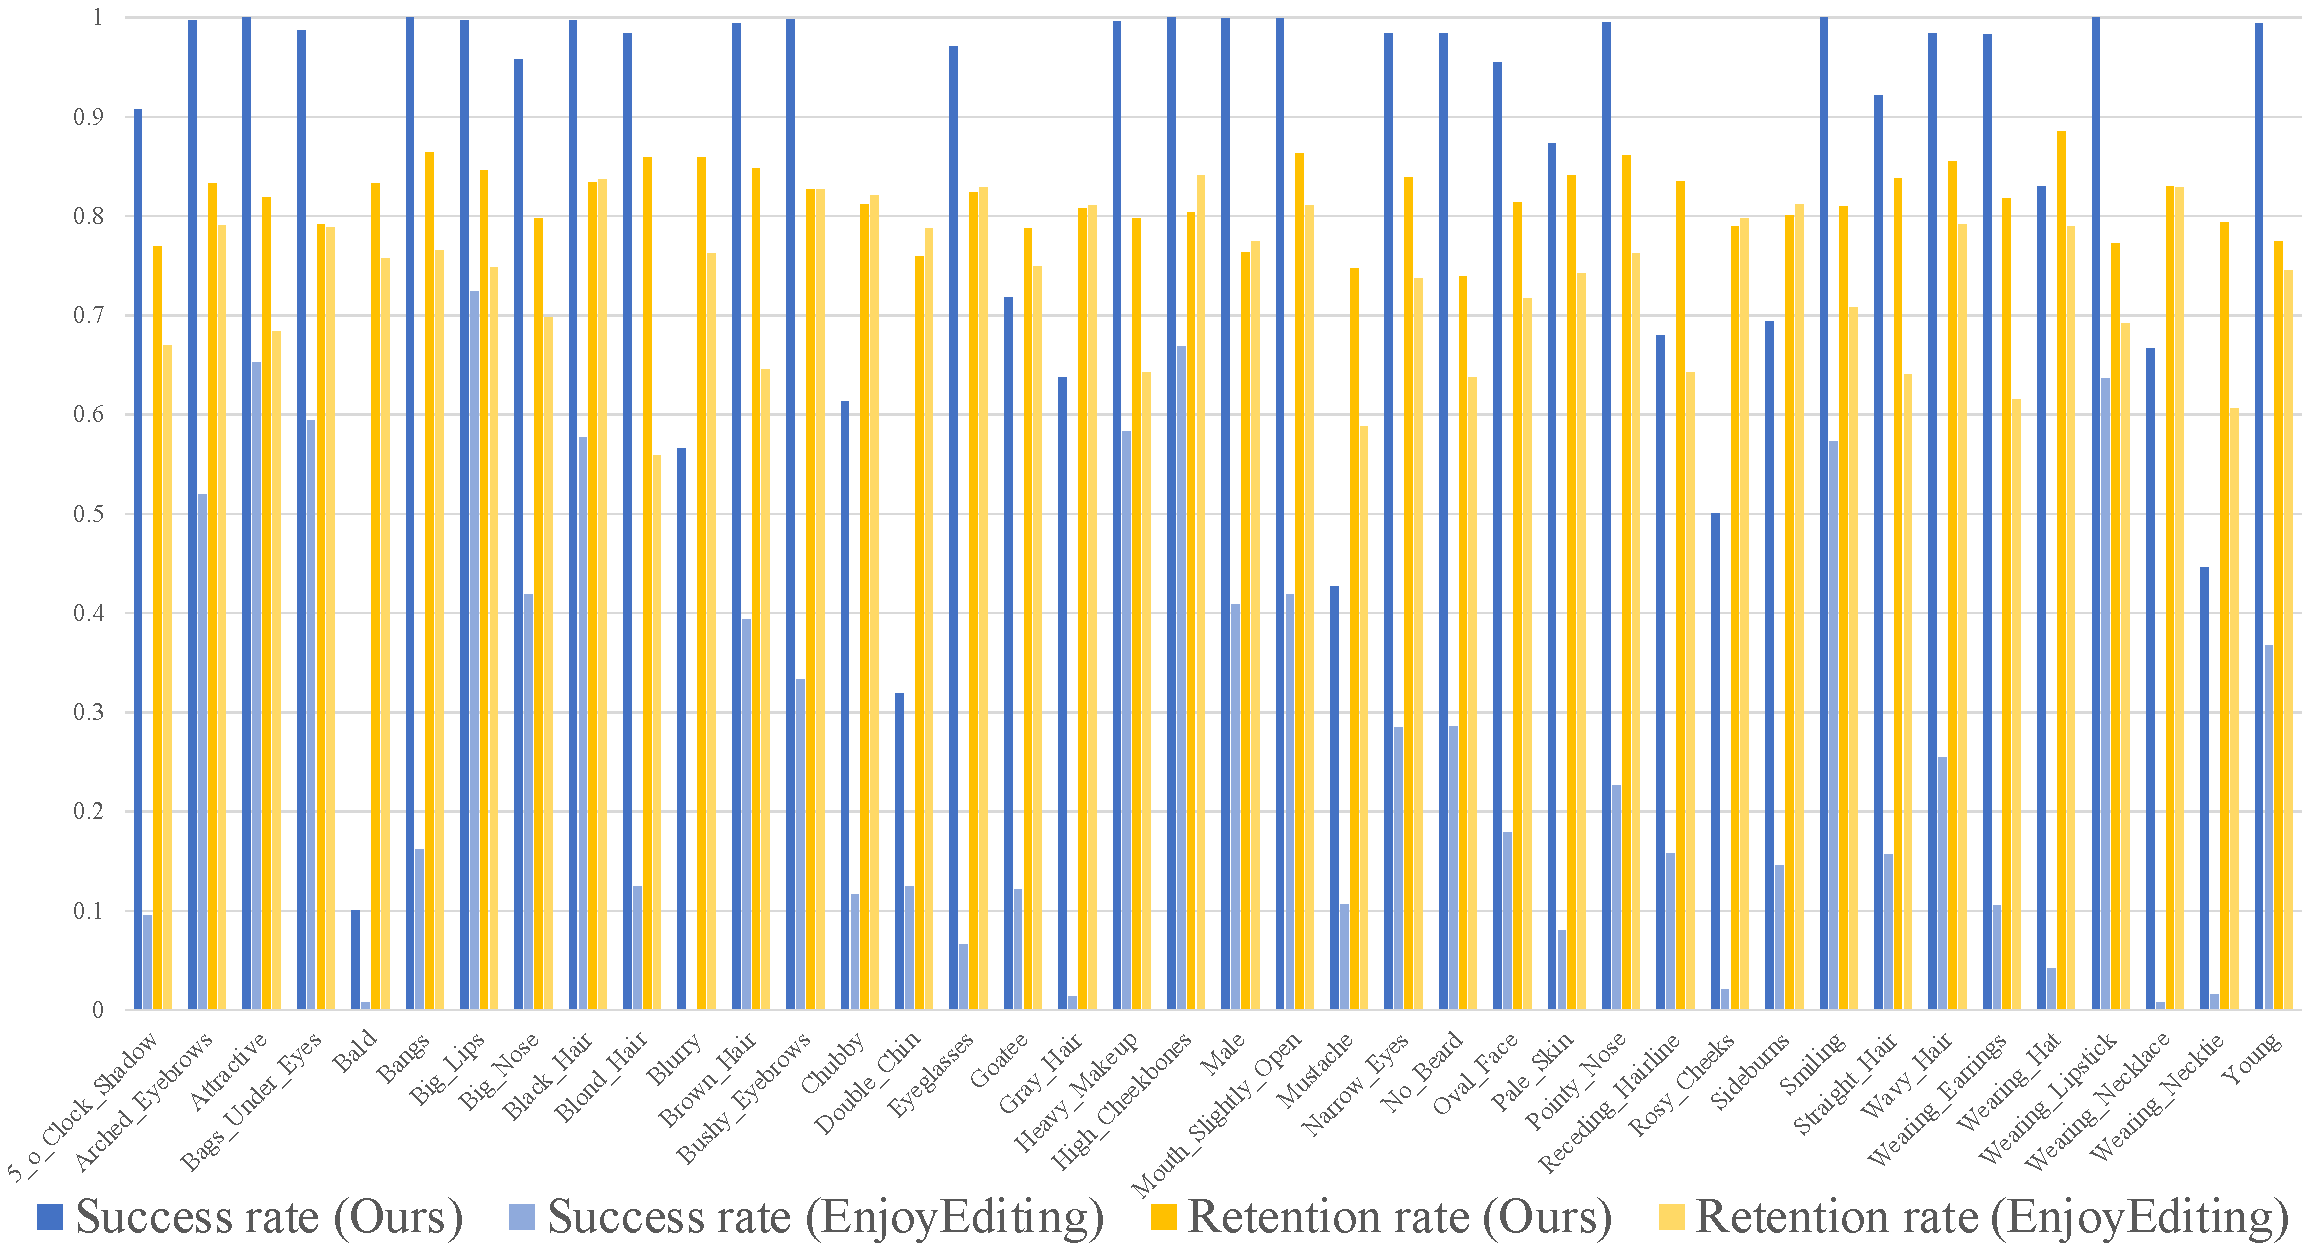
\includegraphics[width=1\linewidth]{figures/ACGAN/excel_histogram.pdf}
    \end{center}
    % \caption{Comparisons of attribute editing accuracy. EnjoyEditing achieves better performance than InterfaceGAN, we only compare our method with EnjoyEditing due to limited space. Please zoom-in for details.}
    \caption{单属性编辑成功率和保留率的的比较}
    \label{fig:histogram}
\end{figure}

我们通过用户调研进一步评估复合属性编辑分数 $\delta$ (属性编辑的成功率)和身份保留分数(即属性编辑的过程中人物身份是否发生变化,是否变成了另外一个人) $\epsilon$。对于我们的 ACGAN,我们首先生成所有属性变量 $0.5$ 的 图像$I_0$,然后我们在原属性变量上减少年龄、黑发、棕发 并增加 灰发(大部分属性值的变化量为$0.3$ )生成 $I_1$。注意属性值是累加的,所以我们在$I_1$的属性代码上增强微笑、浓眉和大鼻子属性,生成$I_2$。 我们生成 $I_3$ 的方式与生成$I_2$时类似。 对于基准方法~\cite{interfacegan}~\cite{iclr2021},我们通过随机抽样隐变量生成$I_0$,并通过隐空间向量算法,以类似属性变化累加的方式生成$\{I_1, I_2, I_3\}$。

我们在图~\ref{fig:questionnaire}中展示了一些生成的人脸图像序列$\{I_0, I_1, I_2, I_3\}$。对于三种不同方法的,我们要求用户回答以下问题:

\begin{enumerate}
\item 图像对 $\{I_0, I_1\}$ 是否满足“更年老”、“更少黑头发”、“更少金发”、“更多白头发”的属性变化?

\item 忽略上题描述的属性变化, $\{I_0, I_1\}$ 中的人物是否是同一个人?

\item 图像对 $\{I_1, I_2\}$ 是否满足“更多微笑”、“更浓密的眉毛”和“更大的鼻子”的属性变化?

\item 忽略上一个问题描述的属性变化,图像对 $\{I_1, I_2\}$ 中的人物是否是同一个人?

\item 图像对$\{I_2, I_3\}$是否满足“更瘦”、“更少双下巴”、“脸更圆”的属性变化?

\item 忽略上题描述的属性变化,图像对 $\{I_2, I_3\}$ 中的人物是否是同一个人?
\end{enumerate}

% For our ACGAN, we first generate $I_0$ with all attributes set to $0.5$, then we reduce \textit{young}, \textit{black hair}, \textit{blond hair} and increase \textit{gray hair} (by $0.3$ mostly) on attribute code of $I_0$ to generate $I_1$. Note that the attribute values are added in an accumulative manner, so we add \textit{smile bushy} and \textit{big nose} on attribute code of $I_1$ to generate $I_2$. The way we adopt to generate $I_3$ is similar to $I_2$. For baselines~\cite{interfacegan}~\cite{iclr2021}, we generate $I_0$ by randomly sampling latent code, and generate $\{I_1, I_2, I_3\}$ through latent space arithmetic but also in an accumulative manner.

% We present some generated face image sequences $\{I_0, I_1, I_2, I_3\}$ in Fig.~\ref{fig:questionnaire}. For each pair in $\{(I_0, I_1), (I_1, I_2), (I_2, I_3)\}$ of all three different methods, we have the following questions:

% \begin{enumerate}
% \item Does the image pair $\{I_0, I_1\}$ satisfy the property changes of "older", "less black hair", "less blond hair" and "more gray hair"?

% \item Ignoring the attribute changes described in the previous question, does the image pair $\{I_0, I_1\}$ have the same identity?

% \item Does the image pair $\{I_1, I_2\}$ satisfy the property changes of "more smiling", "more bushy eyebrows" and "bigger nose"?
% attribute
% \item Ignoring the property changes described in the previous question, does the image pair $\{I_1, I_2\}$ have the same identity?

% \item Does the image pair $\{I_2, I_3\}$ satisfy the property changes of "less chubby", "less double chin" and "less oval face"?

% \item Ignoring the attribute changes described in the previous question, does the image pair $\{I_2, I_3\}$ have the same identity?
% \end{enumerate}

\begin{figure}[!t]
    \begin{center}
         \includegraphics[width=1\linewidth]{figures/ACGAN/questionnaire_new.pdf}
    \end{center}
    \caption{用户问卷样本}
    \label{fig:questionnaire}
\end{figure}

用户调研结果如表~\ref{tb:userstudy}所示。每个单元格中的两个数字分别为属性编辑得分和加权身份保持得分。A组是\{-年轻,-黑色头发,-金色头发,+灰色头发\},B组是\{+微笑,+浓密眉毛,+大鼻子\},C组是-\{-胖,-双下巴,-鹅蛋脸\}。对于身份保留,考虑到这个分数只有在满足属性编辑时才有意义,我们提出了加权身份保留分数 $\epsilon_w = \delta * \epsilon$。 每个单元格中的两个数字分别是 $\delta$ 和加权的 $\epsilon_w$。 我们的方法在编辑精度和加权身份保留两方面均显示出在复合属性编辑上的优越性。 
% We further evaluate composite attributes editing score $\delta$ and identity preserving score $\epsilon$ by user study.  For identity preserving, this score is meaningful only when attributes editing is satisfied. Based on this, we propose weighted identity preserving score $\epsilon_w = \delta * \epsilon$. The evaluation results are reported in Table.\ref{tb:userstudy}. The two numbers in each cell are $\delta$ and weighted $\epsilon_w$, respectively. Our method shows superiority on composite attributes editing in both editing precision and weighted identity preserving evaluations. We provide more details of the user study in supplementary material.

\begin{table}
    \caption{复合属性编辑的定量评价}
    % \caption{Quantitative evaluation of composite attributes editing. The two numbers in each cell are attribute editing score and weighted identity preserving score respectively. GROUP A is \{-Young, -Black Hair, -Blond Hair, +Gray Hair\}, GROUP B is \{+Smile, +Bushy Eyebrows, +Big Nose+\}, GROUP C is \{-Chubby, -Double Chin, -Oval Face\}.}
    \renewcommand\arraystretch{0.8}
        \begin{center}
        % {lC{3.4cm}C{3.3cm}C{2.8cm}}
        \begin{tabular}{cccc}
        \toprule
        & \makecell[c]{A组} & \makecell[c]{B组} & \makecell[c]{C组}\\
        & $\delta$ \space\space\space\space\space\space $\epsilon$  & $\delta$ \space\space\space\space\space\space $\epsilon$  & $\delta$ \space\space\space\space\space\space $\epsilon$ \\
        \midrule
        InterFaceGAN &$45.4$ \space\space $34.0$ &$52.8$\space\space $35.5$&$60.3$ \space\space $40.6$ \\
        \specialrule{0em}{1pt}{1pt}
        EnjoyEditing &$65.9$ \space\space $49.1$ &$76.0$ \space\space $59.1$&$58.9$ \space\space $46.6$ \\
        \specialrule{0em}{1pt}{1pt}
        Ours &$\textbf{87.7}$ \space\space $\textbf{70.6}$ &$\textbf{84.3}$ \space\space $\textbf{68.5}$&$\textbf{85.9}$ \space\space $\textbf{65.0}$ \\
        \bottomrule
        \end{tabular}
        \end{center}
        \label{tb:userstudy}
\end{table}


\subsubsection{所有属性的编辑}
以前的有监督的隐空间编辑方法仅能在CelebA 数据集的少数 ($<$4) 种属性起作用。我们的方法在这方面取得了很大进展,能够编辑生成样本的所有 40 种属性。具体的做法是,我们将所有属性值都初始化为 $0.5$,对于每种属性编辑,只需将该属性值修改为1,同时保持其他属性值和原始内容值不变。 图~\ref{fig:40Attributes}展示了CelebA 数据集中所有 40 种属性的编辑样本。
我们的模型能够很好地解耦大多数属性,除了四个“穿戴性质”的属性:戴项链、戴领带、戴耳环和戴着帽子,这证明了所提出的正交属性空间的有效性,
在分析这些穿戴属性的比例时,我们发现对这些属性的编辑失败并不是由数量引起的。例如,同为穿戴性质属性,眼镜在数量比例上可与其他四种穿戴性质接近,但属性编辑的结果却合理的多。这可能是因为眼镜在面部的大小和位置是相对固定的,而其他穿戴性质属性则不是,这使得“眼镜”的属性编辑比其他穿戴性质属性的编辑更容易学习。
% Previous supervised direction searching methods are only compatible with few ($<$ 4) attributes of the CelebA dataset. Our method has made great progress in this regard, being able to edit all the 40 attributes of the generated samples. Specifically, all the attribute values are initialized to $0.5$. For each attribute editing, we simply modify the editing attribute value to 1 while keep other attribute values and original content values unchanged. Fig.~\ref{fig:40Attributes} demonstrates the effectiveness of the proposed attribute orthogonal space, which empowers our model to well disentangle most attributes except for four "\textit{wearing}" attribute: wearing necklace, wearing necktie, wearing earrings and wearing hat.
% While analyzing the proportion of these wearable attributes, we found that the failure editing on these attributes is not caused by quantity. For instance, as a wearable attribute, eyeglasses are comparable to the other four wearable attributes in the quantity proportion but present reasonable results. This might because the size and the position of the eyeglasses in the face are relatively fixed, while the other wearable items are not, which makes the eyeglasses attribute editing is easier to learn than other wearable attributes.

\begin{figure}[!t]
    \begin{center}
       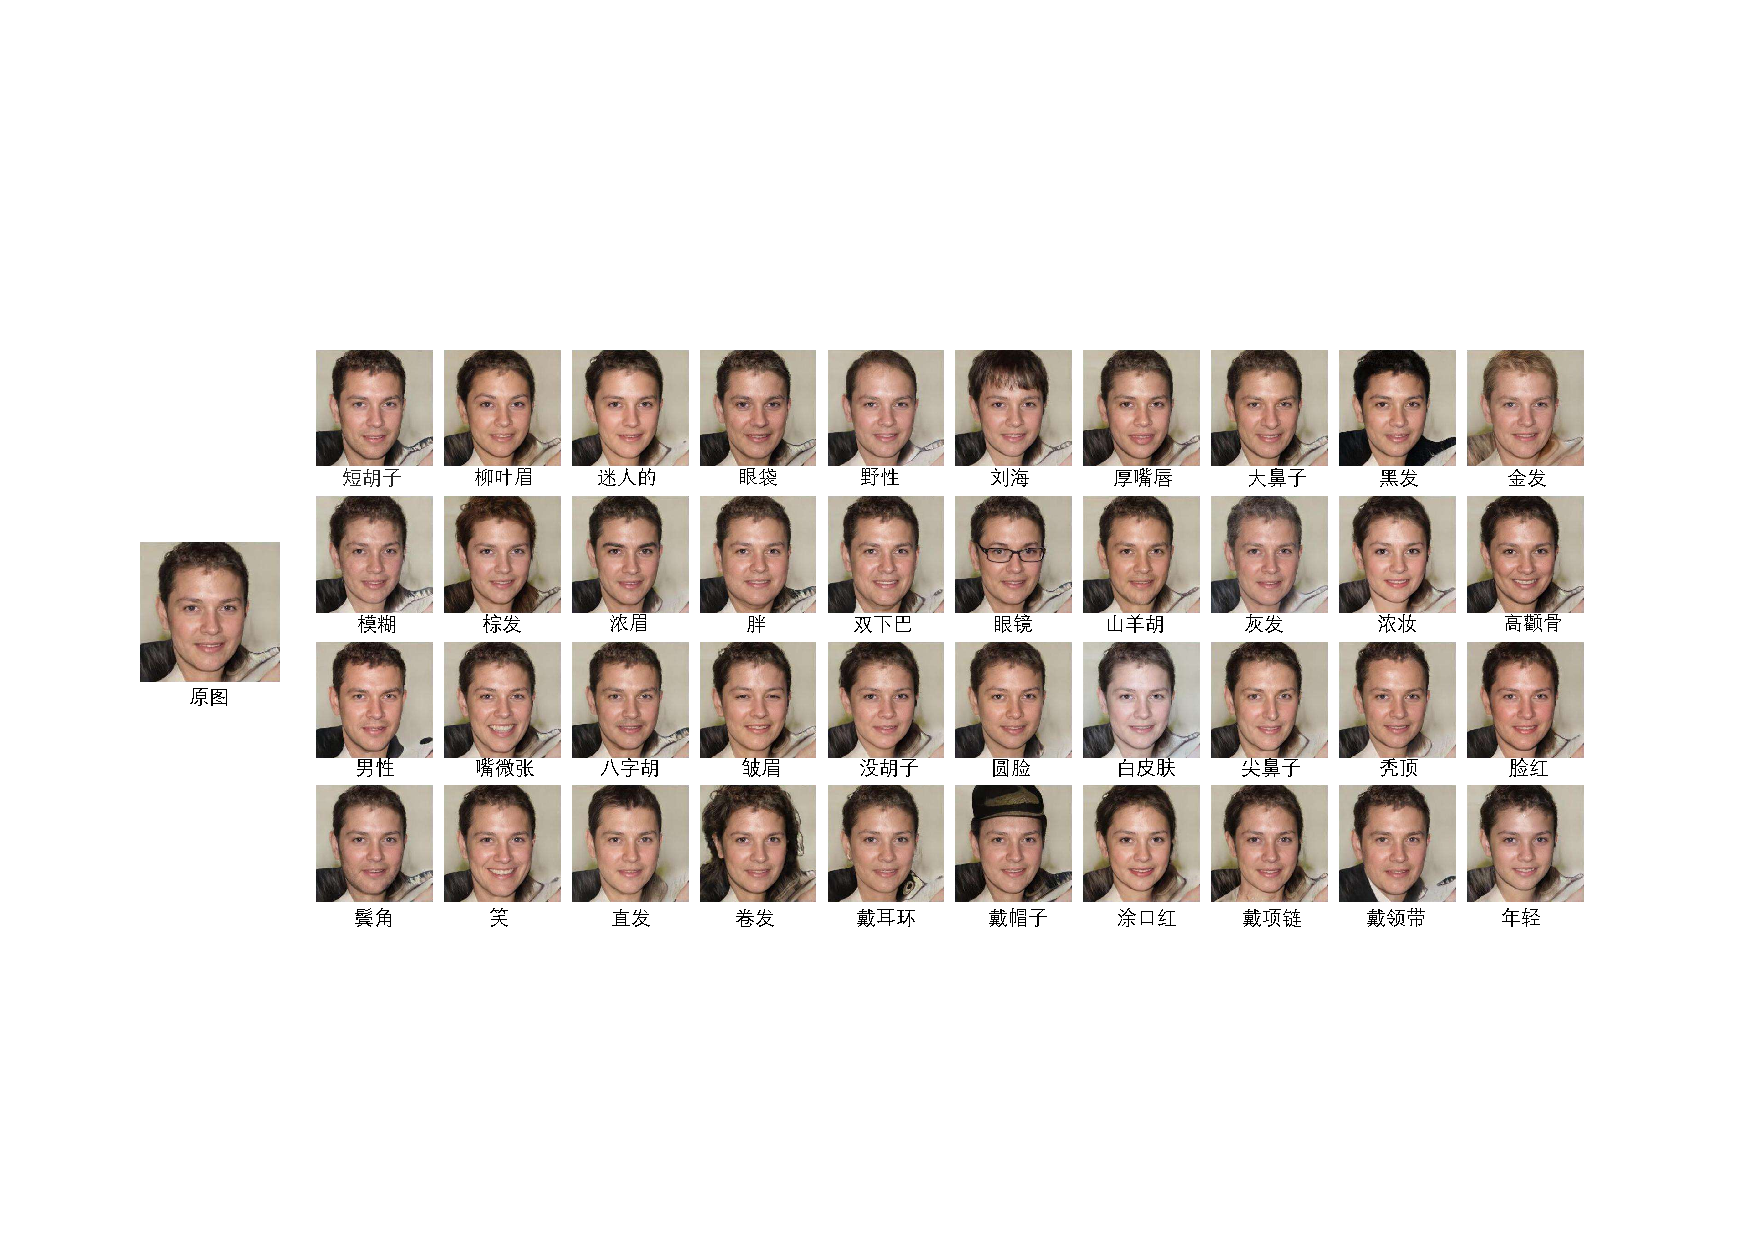
\includegraphics[width=0.9\linewidth]{figures/ACGAN/40Attributes.pdf}
    \end{center}
    \caption{40种属性的编辑}
    % \caption{Edited samples of all 40 attribute in CelebA dataset. The original image is generated under all attribute values equal to 0.5. For each attribute editing, we simply increase that attribute value to 1 and keep content values and other attribute values unchanged.}
    \label{fig:40Attributes}
\end{figure}

\subsubsection{$C$和$R$的分析}
我们将 $[0,1]$ 分成 20 个相等的间隔,并在 FFHQ 数据集上绘制属性 \textit{smiling} 得分的频率直方图。 如图~\ref{fig:quantization}(c)所示,sigmoid会将属性分类器$C$的输出推向接近0或1。$\mathcal{A}$训练的属性回归器也生成大部分预测值接近 到 0 或 1,如图~\ref{fig:quantization}(d)所示。相反,我们由 $\hat{\mathcal{A}}$ 训练的属性回归器 $R$ 产生了如图~\ref{fig:quantization}(e)所示的更合理的从 0 到 1 的连续值。 
% We divide $[0,1]$ into 20 equal intervals and plot frequency histogram of attribute \textit{smiling} score on FFHQ dataset. As shown in Fig.~\ref{fig:quantization}(c), sigmoid will push output of attribute classifier $C$ close to 0 or 1. Attribute regressor trained by $\mathcal{A}$ also generates most prediction values close to 0 or 1 as demonstrated in Fig.~\ref{fig:quantization}(d). On the contrary, our attribute regressor $R$ trained by $\hat{\mathcal{A}}$ produces more reasonable continuous values from 0 to 1 as in Fig.~\ref{fig:quantization}(e). We provide more analysis in the supplementary material.

\subsection{自然风景属性编辑相关实验}

\subsubsection{定性比较}
在 \cite{iclr2021} 之后,我们将我们的 ACGAN 与图像到图像方法 CycleGAN~\cite{cyclegan}、RelGAN~\cite{relgan} 和 DRIT++~\cite{drit++} 进行比较,如图~\ref{fig:sceneComparison}。 我们根据属性值将 Transient Attributes 数据集分为两部分:\textbf{A} 部分(属性值 $>$ 0.5)和 \textbf{B} 部分(属性值 $\leq$ 0.5)。 这些方法是通过从 \textbf{A} 部分到 \textbf{B} 部分的转换图像从头开始训练的,反之亦然。
如图~\ref{fig:sceneComparison}所示,与其他方法相比,我们的ACGAN准确地改变了原始图像的属性,这表明我们的模型在自然属性编辑方面表现良好。
% Following \cite{iclr2021}, we compare our ACGAN with image-to-image methods CycleGAN~\cite{CycleGAN2017}, RelGAN~\cite{relgan}, and DRIT++~\cite{drit++} in Fig.~\ref{fig:sceneComparison}. We split Transient Attributes dataset into two parts based on attribute value: \textbf{A} part (attribute value $>$ 0.5) and \textbf{B} part (attribute value $\leq$ 0.5). These methods are trained from scratch by translation image from \textbf{A} part to \textbf{B} part and vice versa.
% As shown in Fig.~\ref{fig:sceneComparison}, compared with other methods, our ACGAN accurately change the attributes of the original images, which suggests that our model performs well in natural attributes editing.

\begin{figure}[t]
    \begin{center}
         \includegraphics[width=0.5\textwidth]{figures/ACGAN/Scenecomparison.pdf}
    \end{center}
    \caption{自然场景单属性编辑对比}
    \label{fig:sceneComparison}
\end{figure}

由于自然图像的属性易于观察,我们对自然场景合成进行连续属性编辑。与人脸合成类似,ACGAN 在编辑自然场景属性(即“夜晚”、“云”、“雾”、“冬天”和“晴天”)方面也表现出卓越的性能。 我们在图~\ref{fig:scene}中展示了我们在自然场景下,每种属性在上图中从 0 增加到 1时的连续属性编辑结果。 受益于正交属性空间,ACGAN实现了自然场景中的准确属性编辑。
% Since the attributes of natural images are easy to observe, we conduct continuous attributes edits on Transient Attributes dataset. Similar to face synthesis, ACGAN also shows superior performance in editing natural scene attributes, i.e., "night", "cloud", "fog", "winter" and "sunny". We present our continuous attribute editing results under natural scene in Fig.\ref{fig:scene}. Benefiting from the orthogonal attribute space, ACGAN achieves accurate attribute editing in natural scenes with regards to image identity preservation.

\begin{figure}
    \begin{center}
         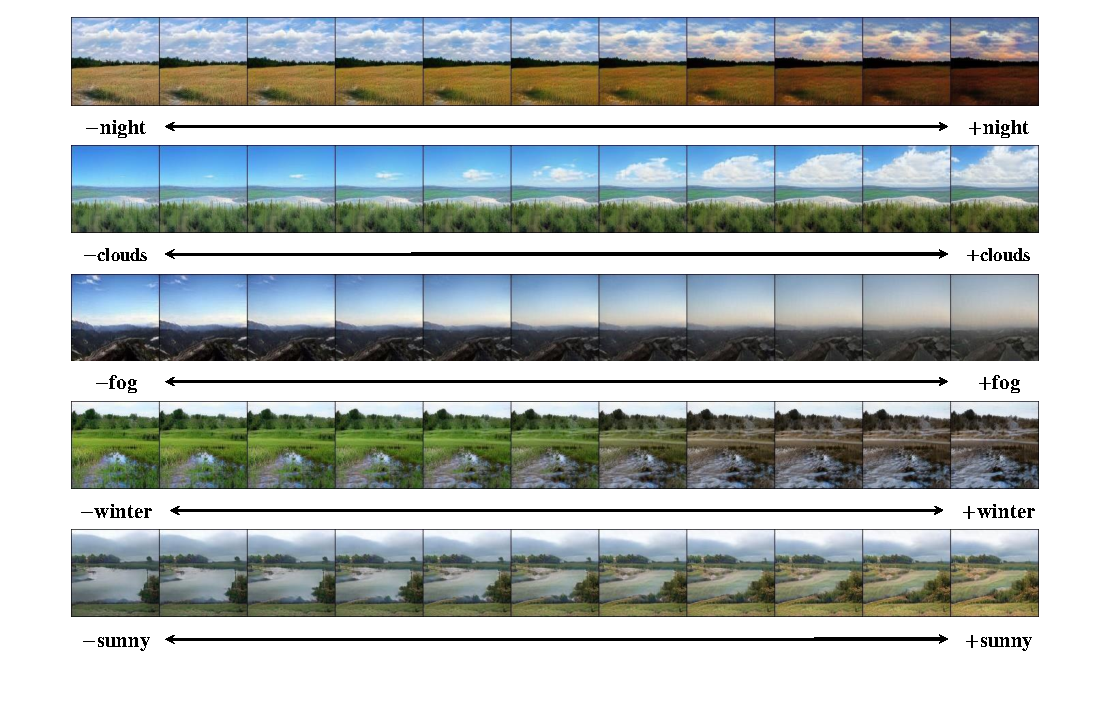
\includegraphics[width=0.85\linewidth]{figures/ACGAN/scene.pdf}
    \end{center}
    \caption{自然场景连续属性编辑}
    % \caption{Edited samples of 5 attributes in Transient Attributes dataset~\cite{scenedataset}. We demonstrate continuous changes in samples with each attribute increasing from 0 to 1 in the above picture.}
    \label{fig:scene}
\end{figure}

\subsubsection{定量比较}
为了定量评估我们的 ACGAN 在控制自然场景合成的属性方面,我们使用我们的 ACGAN 为每种属性生成 $5,000$ 的图像对 $(I_-,I_+)$。 $I_-$ 表示该属性为“关闭”或“负”,反之亦然。 我们在由属性回归器 $R$ 计算的 $(I_-,I_+)$ 之间定义属性增益(Attribute Gain)$AG$:
\begin{equation}
     AG = R(I_+)-R(I_-)。
\end{equation}
属性增益越大,该方法控制属性的能力越强。 为了与图像空间转换方法进行比较,我们使用 DRIT++ 和 RelGAN 生成额外的 $I_+$ 给定输入 $I_-$ 并计算它们之间的属性增益。从表~\ref{tb:attrbute_gain}展示的各个属性的增益对比中,可以看到我们的 ACGAN 的属性增益远高于其他方法,这证明我们的 ACGAN 对控制属性的能力最强。
% To quantitatively evaluate our ACGAN on controlling attributes for natural scene synthesis, we use our ACGAN to generate $5,000$ image pairs $(I_-,I_+)$ for each attribute. $I_-$ means this attribute is "off" or "negative" and vice versa. We define attribute gain between $(I_-,I_+)$ computed by attribute regressor $R$ : attribute gain=$R(I_+)-R(I_-)$. The larger the attribute gain, the stronger the method is in controlling attributes. To compare with image-space translation methods, we use DRIT++ and RelGAN to generate extra $I_+$ given input $I_-$ and compute attribute gain between them. The results are shown in Table~\ref{tb:attrbute_gain}. The attribute gain of our ACGAN is much higher than the other methods, which proves that our ACGAN has the strongest power over controlling attributes. 

\begin{table}[!t]
    \caption{属性增益对比}
    % \caption{The attribute gain of our ACGAN is much higher than the other methods, which proves that our ACGAN has the strongest power over controlling attributes.}
    \renewcommand\arraystretch{0.8}
    \begin{center}
    \begin{tabular}{lccccc}
    %{lC{3.4cm}C{3.3cm}C{2.8cm}}
    \toprule
    & 多云 & 雾 & 冬天 & 夜晚 & 晴天\\
    \midrule
    RelGAN & $0.1271$ & $0.1046$ & $0.1009$ & $0.1692$ & $0.1918$ \\
%   \hdashline
    \specialrule{0em}{1pt}{1pt}
    DRIT++ & $0.1183$ & $0.0177$ & $0.1496$ & $0.1055$ & $0.0736$ \\
%   \hdashline
    \specialrule{0em}{1pt}{1pt}
    \textbf{Ours} & $\textbf{0.3069}$ & $\textbf{0.2656}$ & $\textbf{0.5979}$ & $\textbf{0.2679}$ & $\textbf{0.3192}$ \\
    \toprule
    \end{tabular}
    \end{center}
    \label{tb:attrbute_gain}
\end{table}

\section{其他视觉效果展示}
本节我们将通过不同的实验设置,进一步展示ACGAN强大的图像属性编辑能力。

\subsection{人脸叠加属性编辑}
人脸叠加属性编辑指在一张图片上依次加入多种属性编辑。 如图~\ref{fig:multiAtt}所示,我们将属性变化+年龄、+白头发、+眼镜、+胡子(男性)或+化妆(女性)、+ 瘦
和+笑容依次加入到原始图像中。我们的方法可以在保持人物身份不变的前提下做出准确的属性编辑。


\begin{figure}[!t]
    \centering
    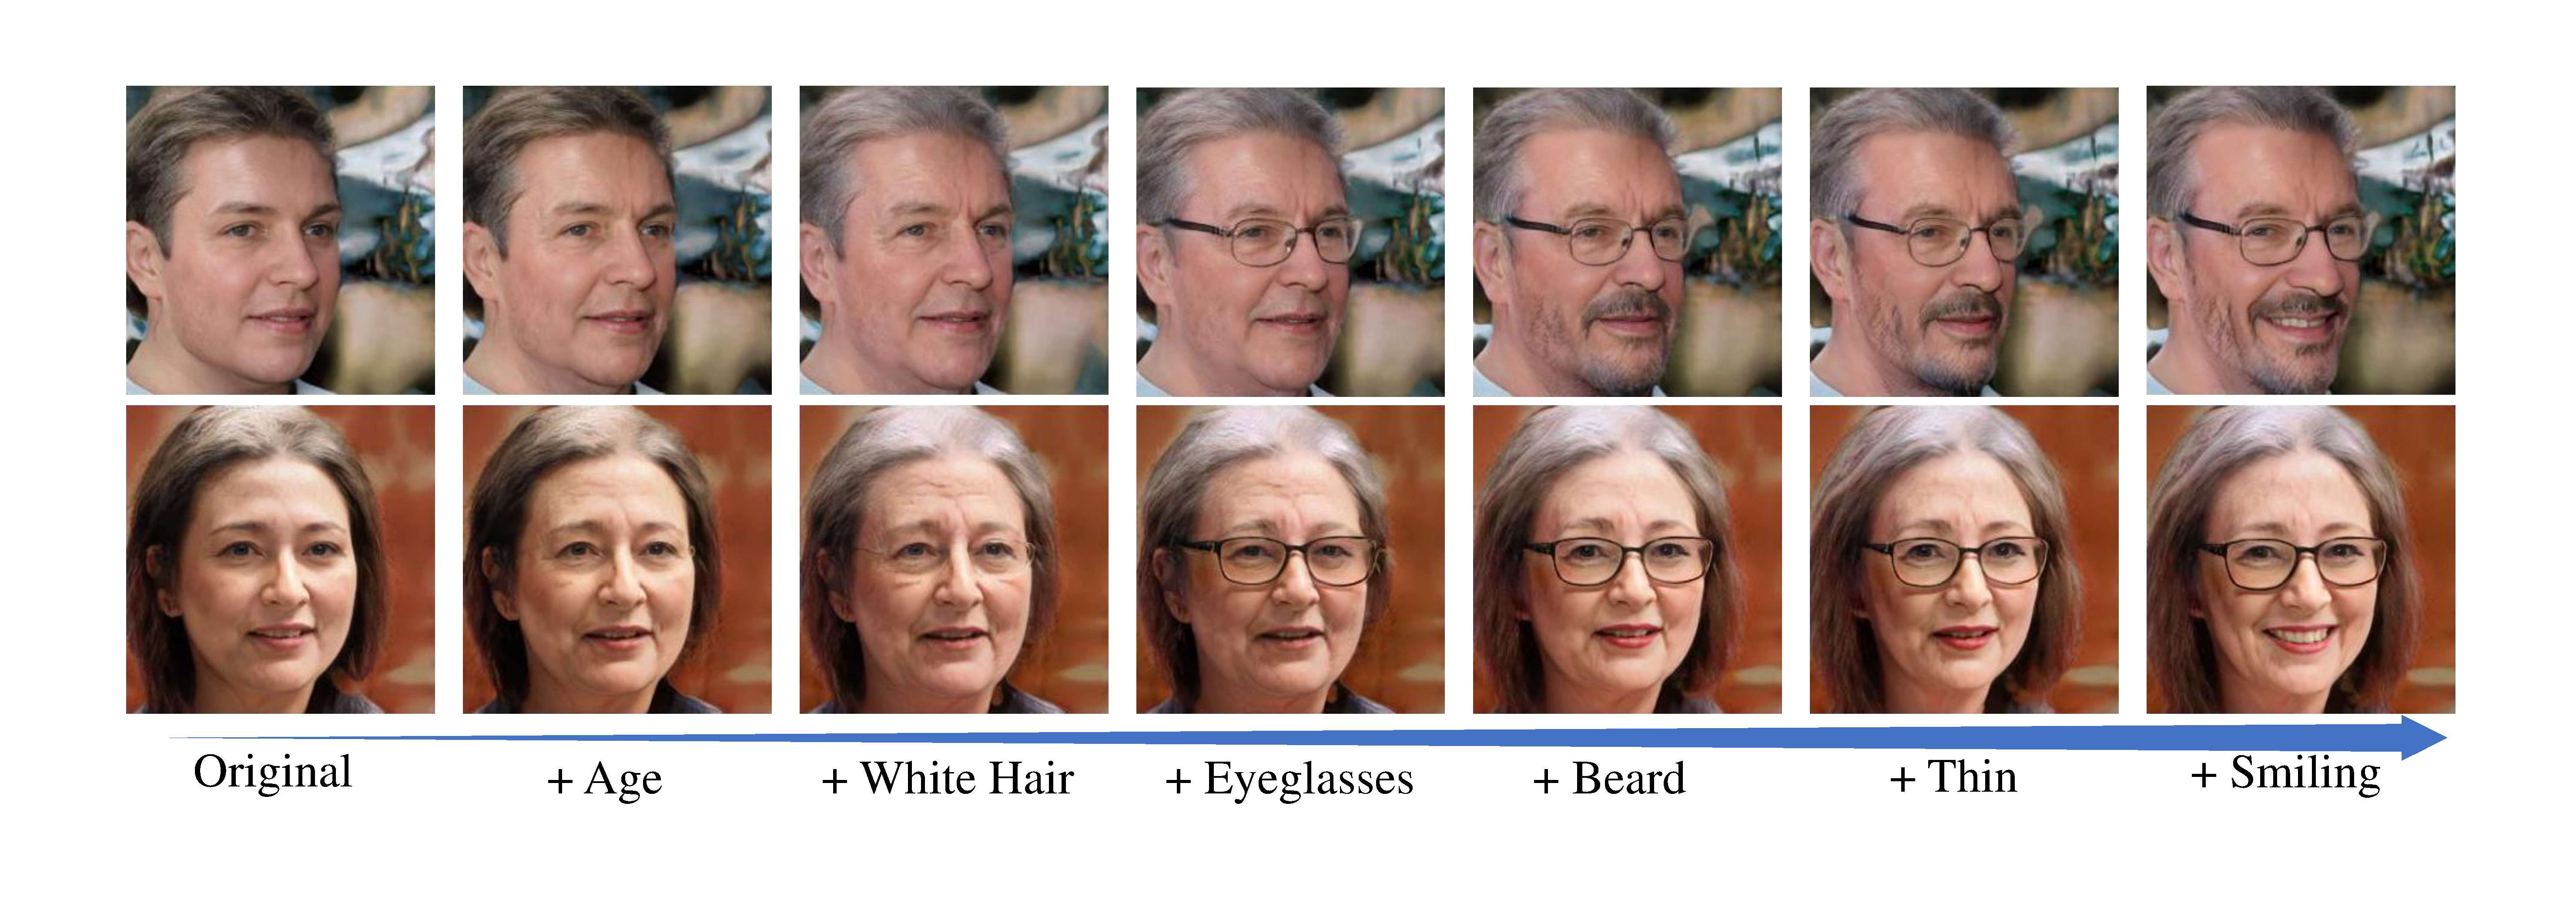
\includegraphics[width=0.8\textwidth]{figures/ACGAN/cover.pdf}
    % \caption{Accumulative attribute editing. We gradually enhance a certain attribute(age, white hair, etc.) from left to right in the portraits. Benefiting from disentanglement between attributes, the editing results are precise and smooth. Zoom in for better view.}
    \caption{人脸叠加属性编辑图}
    \label{fig:multiAtt}  
\end{figure}


我们进一步进行了增强和减弱属性年龄、眼镜、胡子、胖瘦和笑容的实验。实验过程中我们通过性别属性控制生成人物的性别,对于性别为女性的图像我们将胡子属性替换为化妆。 如图~\ref{fig:male}和图~\ref{fig:female}所示,我们的ACGAN可以对多个面部属性进行复杂的编辑。
% Here we show additional results of accumulatively manipulating multiple attributes on face images. The attributes \textit{Age}, \textit{White Hair}, \textit{Eyeglasses}, \textit{Beard}, \textit{Thin} and \textit{Smiling} are added accumulative to the original images. As shown in Fig.~\ref{fig:multiAtt}, our method can generate accurate attribute editing with excellent identity consistency and realistic textures. 
% We further conduct experiments on adding and removing the attributes \textit{Age}, \textit{Eyeglasses}, \textit{Beard}, \textit{Chubby} and \textit{Smiling} in turn to more images with \textit{Male} attribute. For the image with \textit{Female} attribute, we replace the \textit{Beard} attribute with the \textit{Makeup} attribute. As shown in Fig.~\ref{fig:male} and Fig.~\ref{fig:female}, our ACGAN is qualified to complex manipulation on multiple facial attributes.

\begin{figure}[!t]
     \begin{center}
          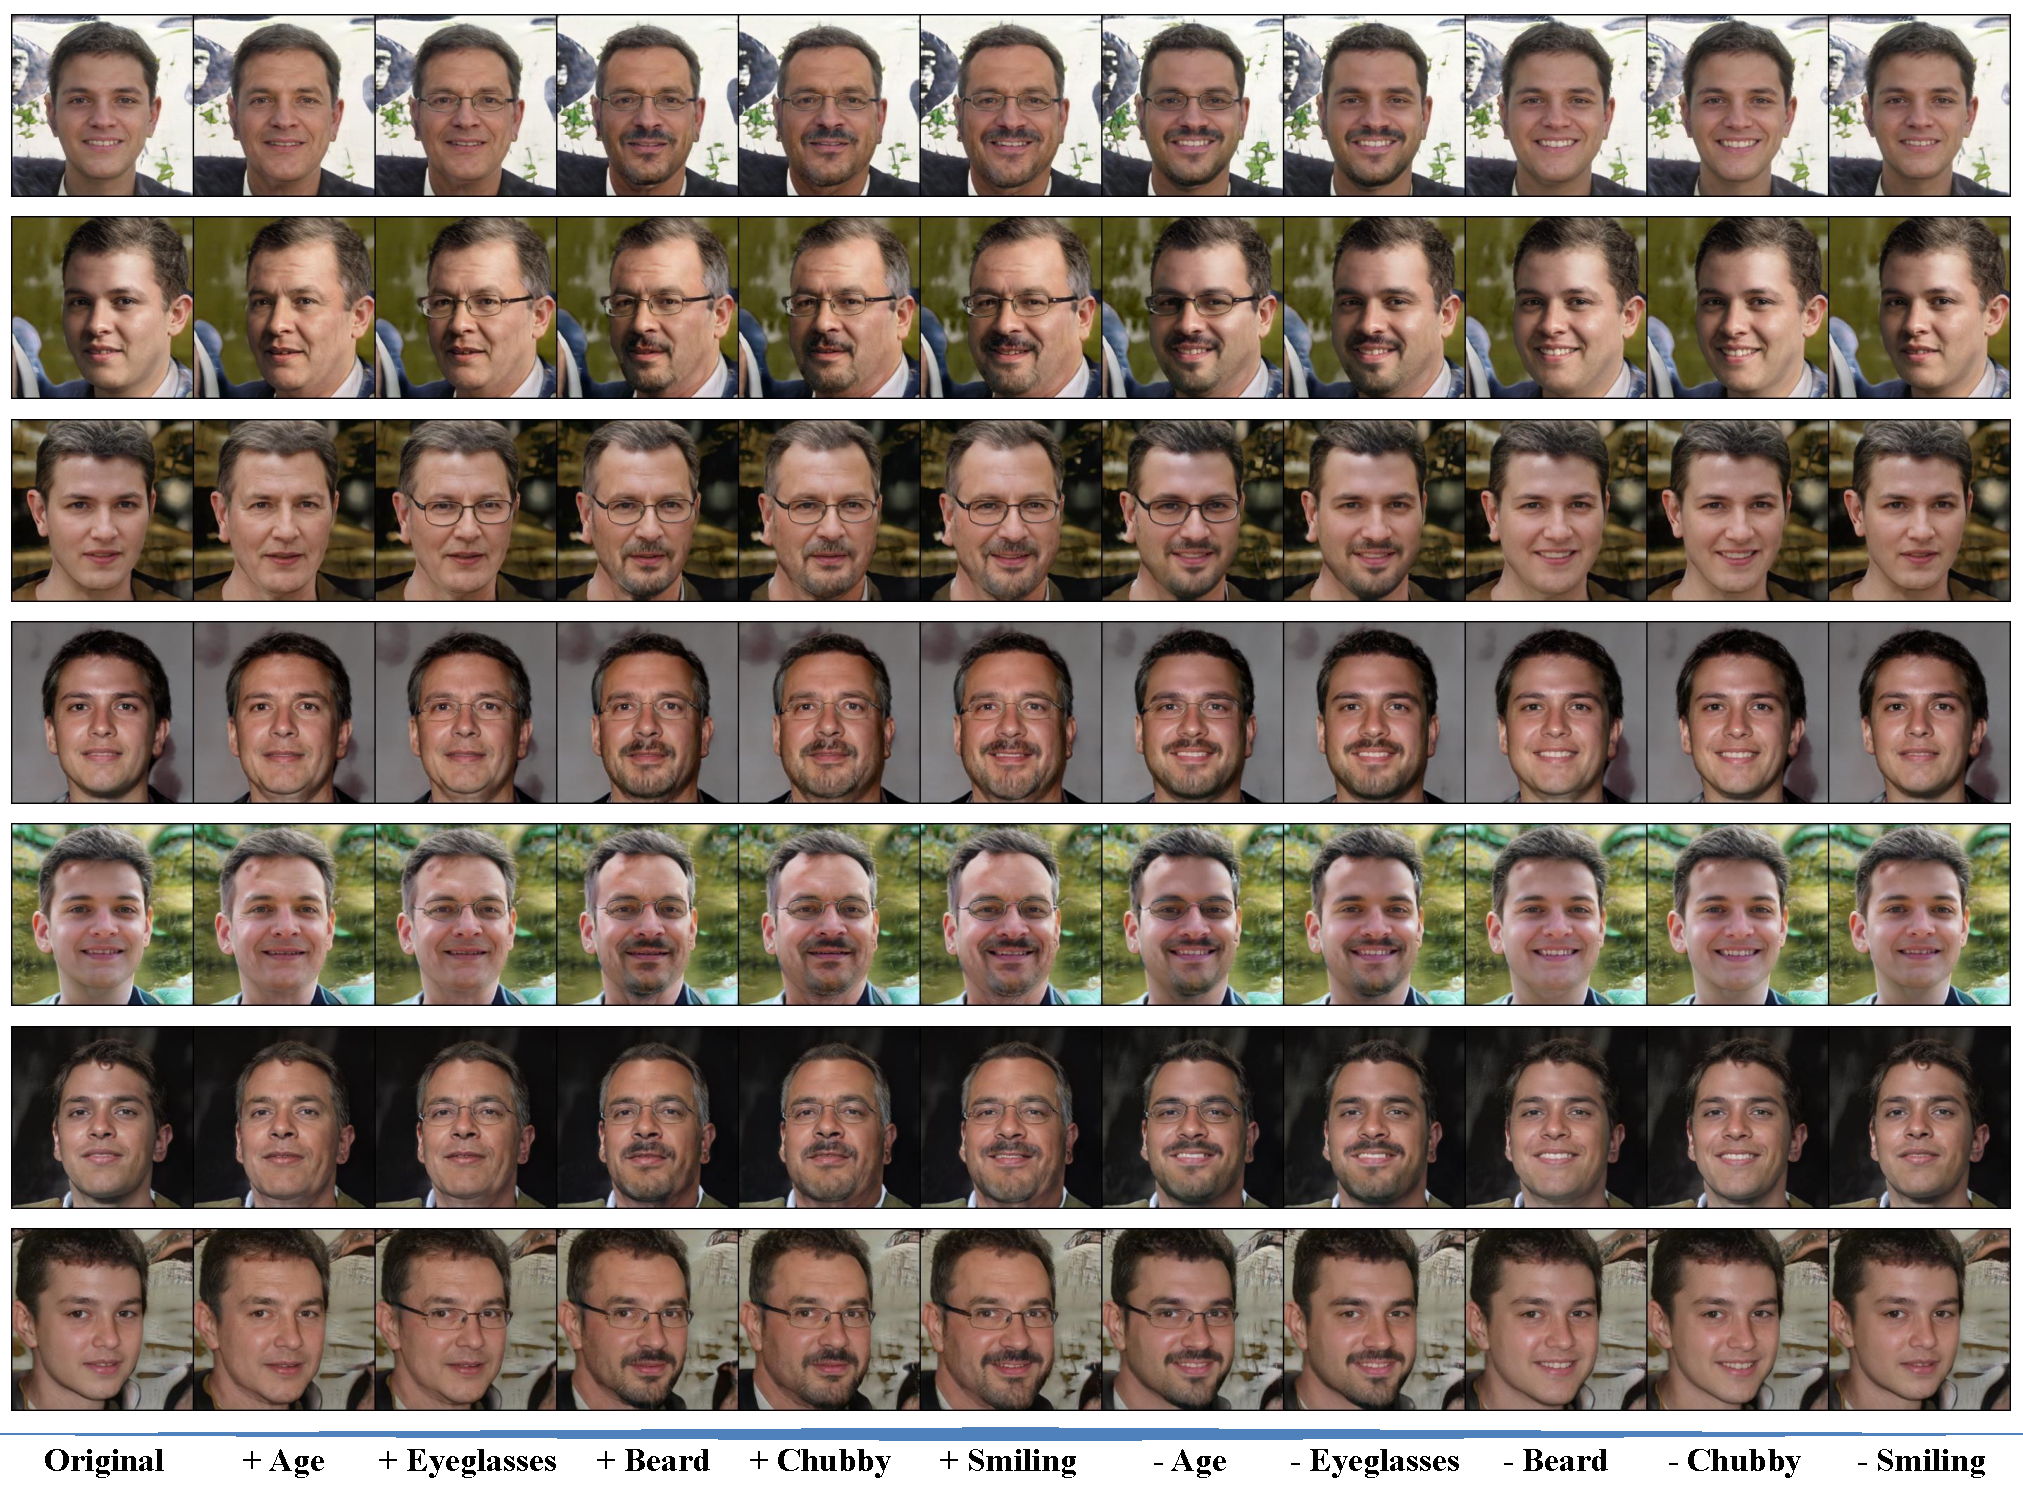
\includegraphics[width=0.8\textwidth]{figures/ACGAN//male.pdf}
     \end{center}
     \caption{男性人脸叠加属性编辑图}
     \label{fig:male}
\end{figure}

\begin{figure}[!t]
     \begin{center}
          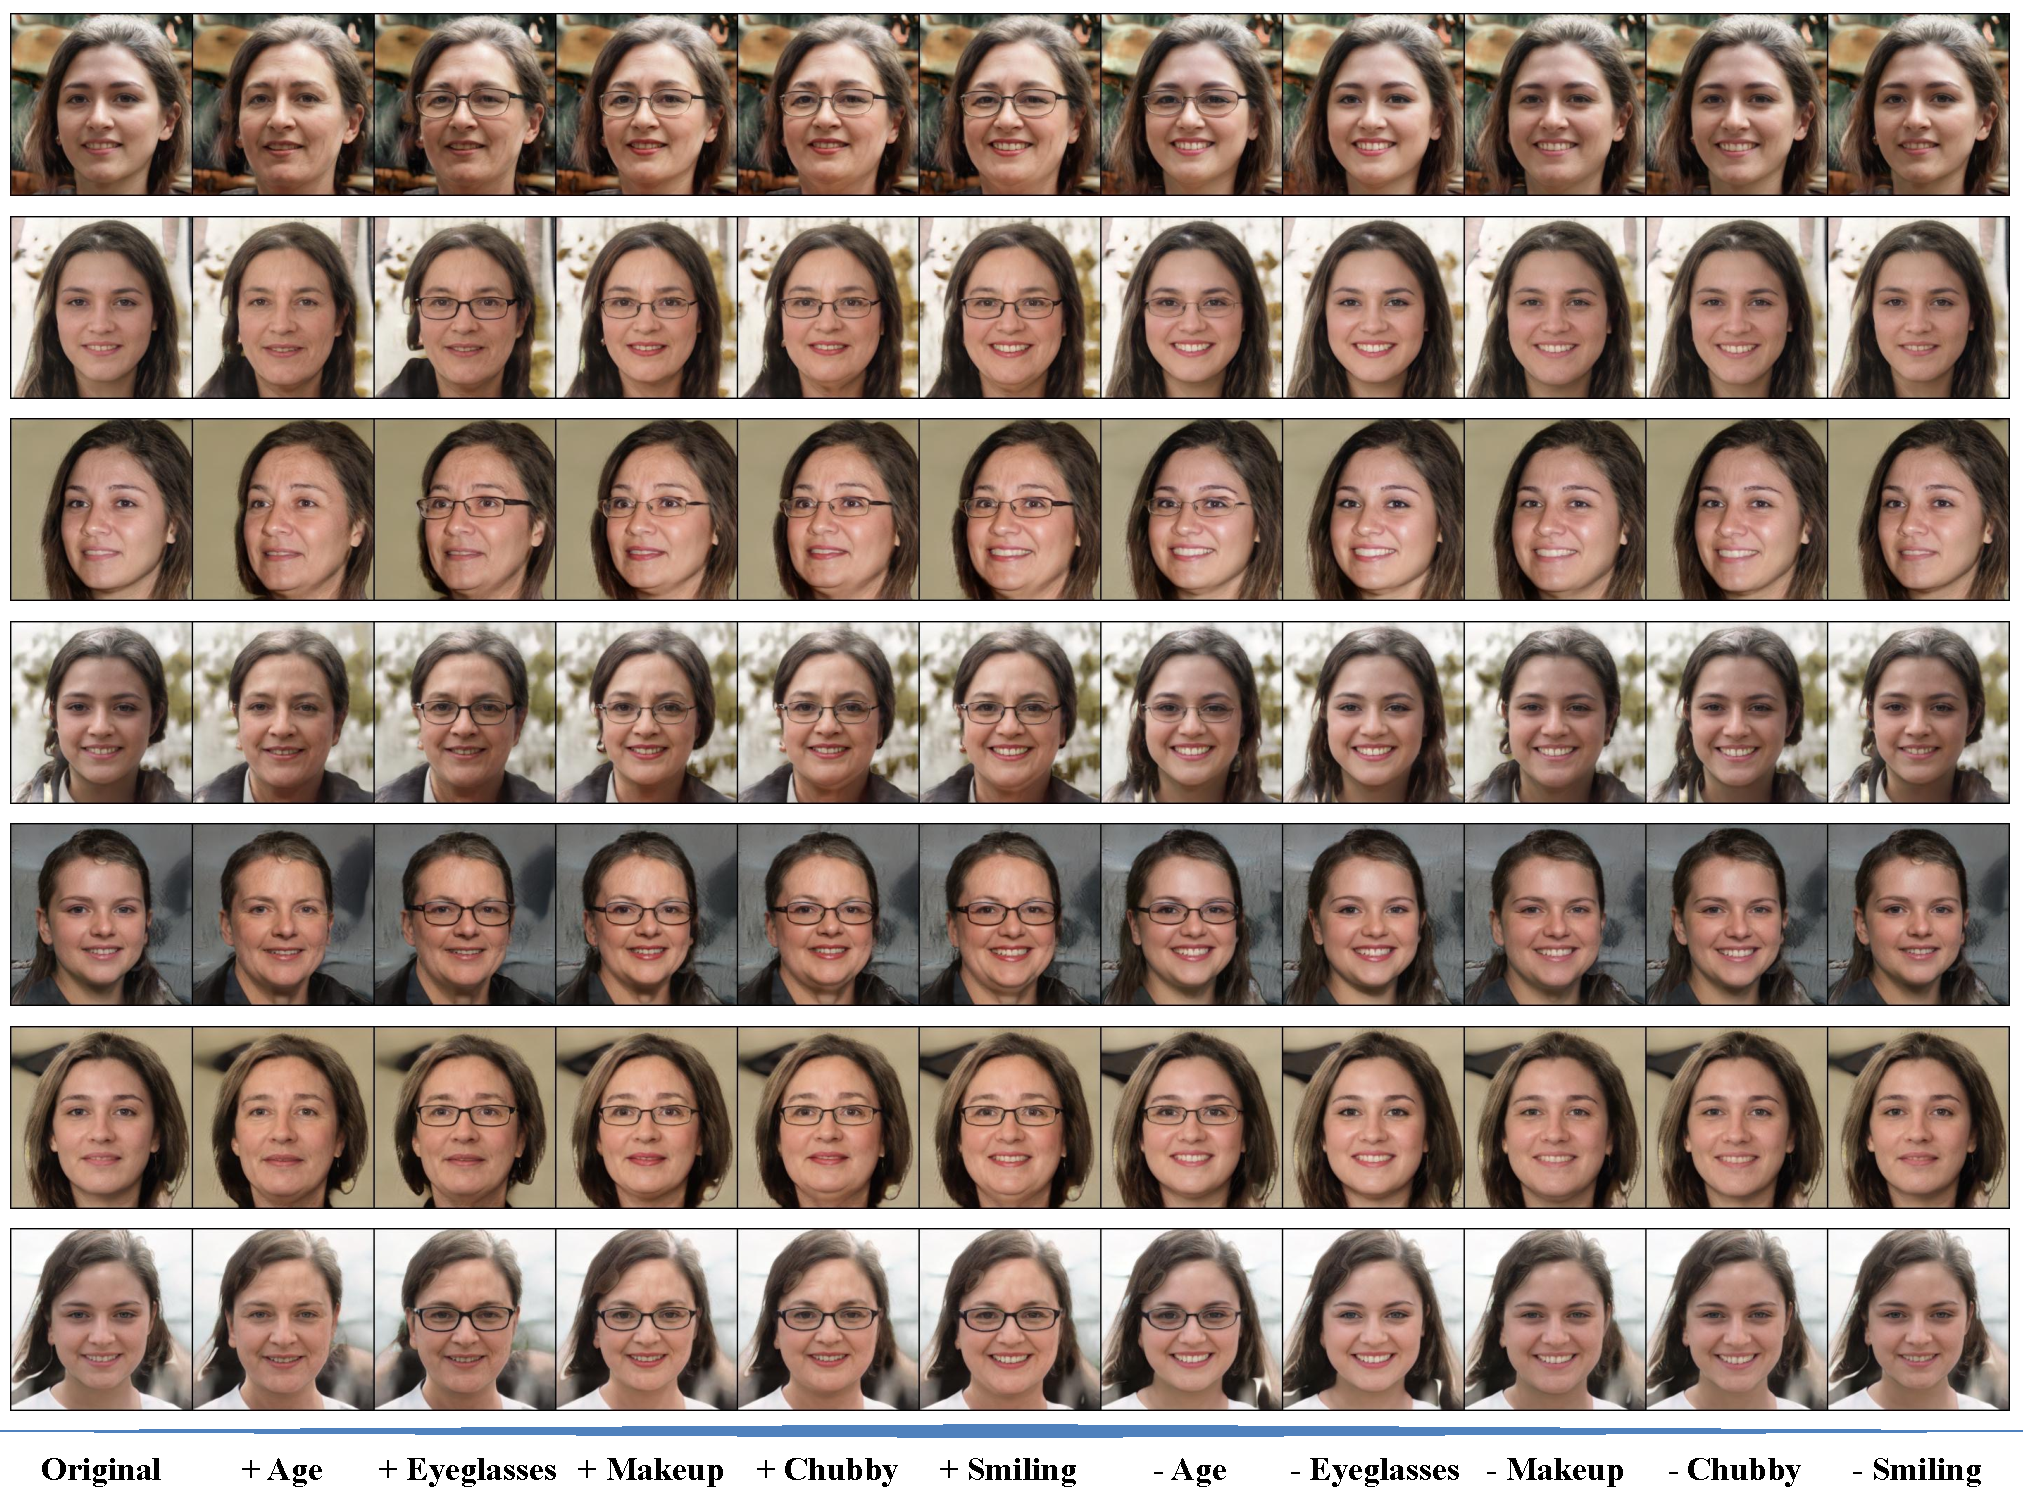
\includegraphics[width=0.8\textwidth]{figures/ACGAN//female.pdf}
     \end{center}
     \caption{女性人脸叠加属性编辑图}
     \label{fig:female}
\end{figure}


\subsection{自然场景复合属性编辑}
我们在图~\ref{fig:sceneMulti} 中展示了ACGAN对自然场景图像进行复合属性(两种属性)编辑的结果。图~\ref{fig:sceneMulti}(a)显示了云和雾的编辑结果,位于(a)左上角的图片既没有雾也没有云,(a)下边的图片包含更多的云和较少的雾,(a)右边的图片往往会产生更多的雾和较少的云;(a)右下角的图片则同时包含较多云和雾。图~\ref{fig:sceneMulti}(b)和(c)遵循类似的规律。就属性解耦来说,三种属性组合:云与雾、云与冬天(季节变化)、云与晴天(天气变化),均实现了肉眼可见的属性解耦。 该实验进一步证明了我们的方法在解耦自然场景属性方面的优越性。
% We present additional results of multiple attributes editing on natural scene images in Fig.~\ref{fig:sceneMulti}. The generated images generated by our method are manipulated on two attributes simultaneously. Fig.~\ref{fig:sceneMulti}(a) shows the results of editing \textit{Clouds} and \textit{Fog}, the top left picture shows neither fog nor clouds, the downwards pictures tend to generate more clouds and less fog, the rightward pictures tend to generate more fog and less clouds; the bottom right picture contains both clouds and fog. Fig.~\ref{fig:sceneMulti}(b) and Fig.~\ref{fig:sceneMulti}(c) show similar performance in disentangling \textit{Clouds} with \textit{Winter} and \textit{Sunny}. This experiment demonstrates the advanced performance of our method in disentangling natural scene attributes. 

\begin{figure}[!ht]
	\begin{center}
		 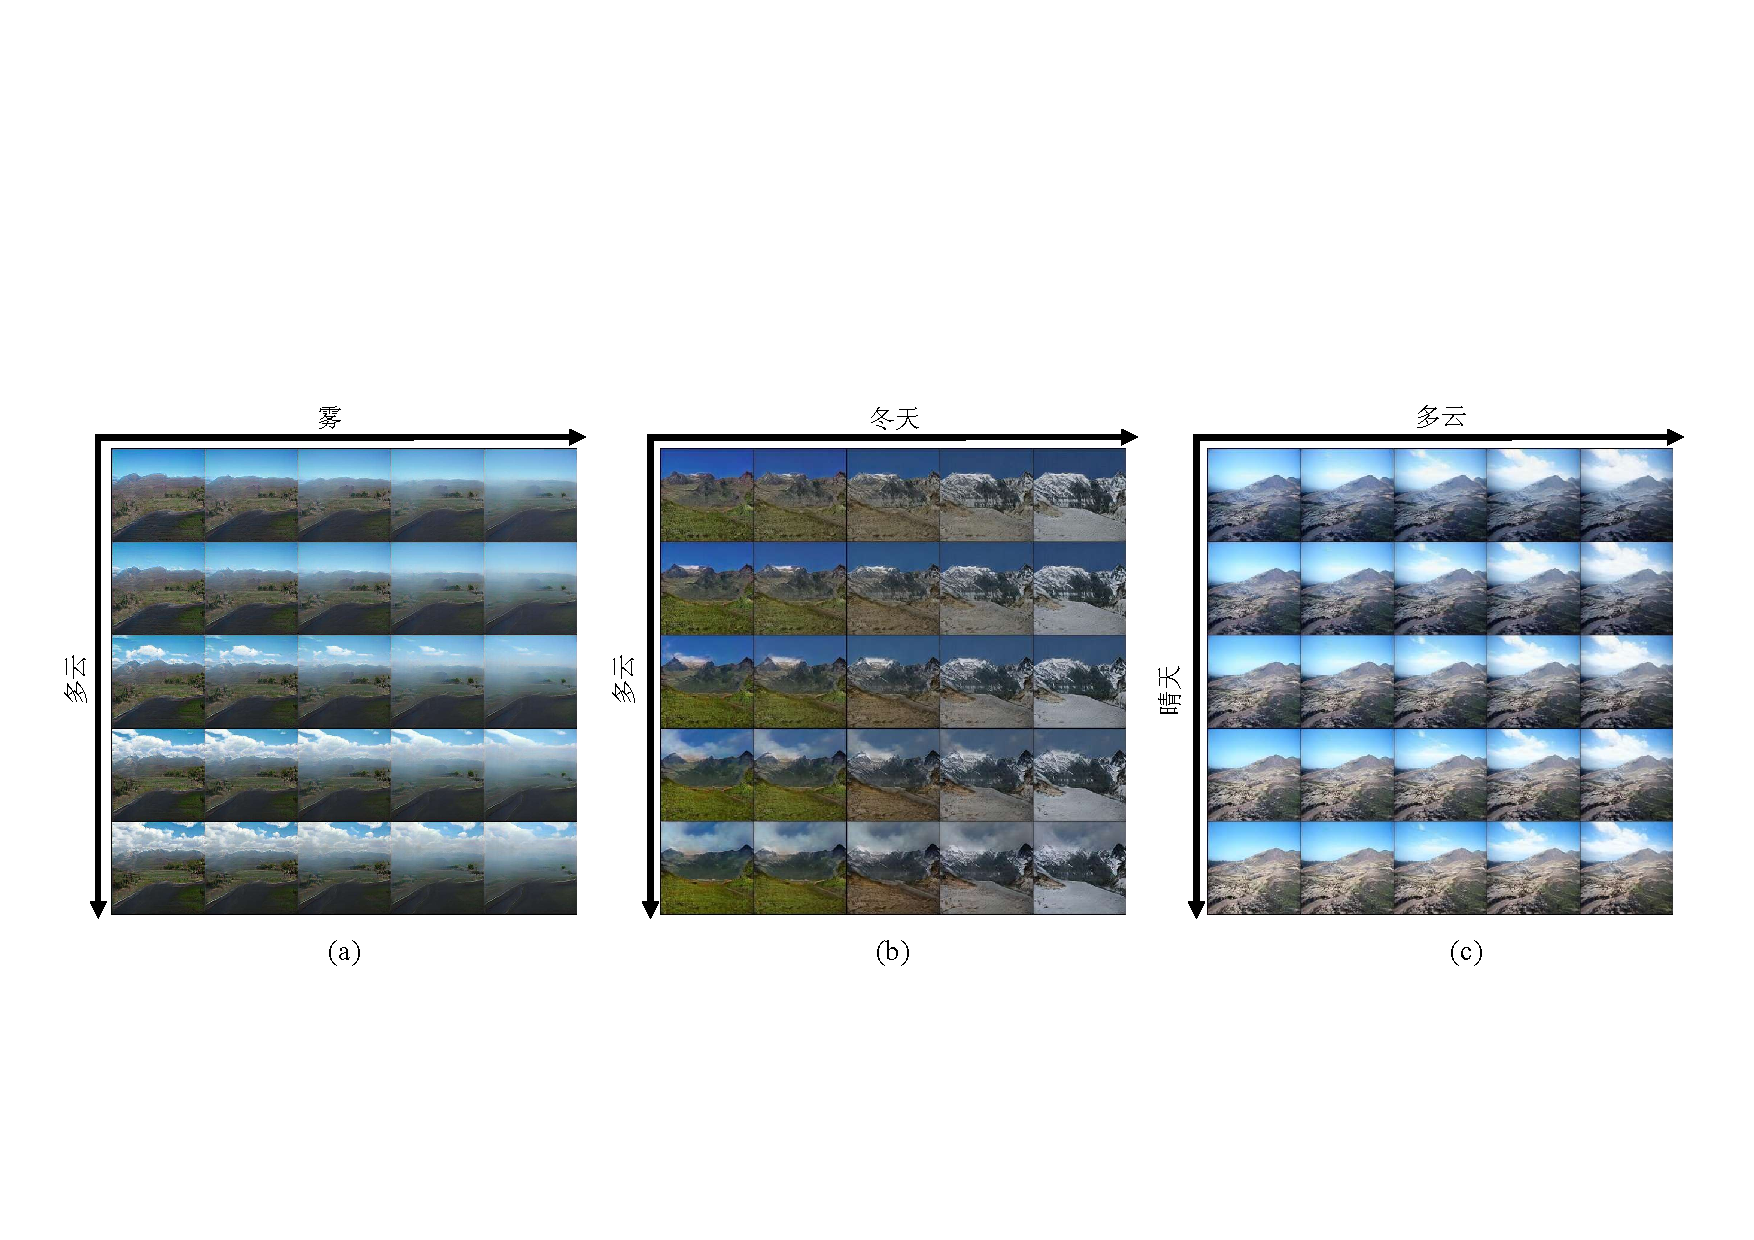
\includegraphics[width=0.8\textwidth]{figures/ACGAN/sceneMulti.pdf}
	\end{center}
	\caption{自然场景复合属性编辑图}
	\label{fig:sceneMulti}
\end{figure}

\section{本章总结}
在这项工作中,为了实现语义解耦的图像编辑,我们提出了一种输入属性与生成图像属性一致的生成式对抗网络ACGAN。 为了在理论上保证每种属性方向与其他方向解耦,我们将属性空间与内容空间隔离,将属性空间投影到正交空间,并提出了属性一致损失来约束输入属性与生成图像属性的属性一致性。为了将我们的方法扩展到所有带有属性标注的数据集,我们进一步提出了一种属性量化策略,将二进制属性标签量化为连续值。 实验证明我们的方法可以在保持图片身份信息不变的前提下,同时且连续地编辑多种属性。
% In this work, we propose a semantic controllable GAN for image attribute editing. To better disentangle each attribute direction from other directions, we isolate an attribute space from the latent space and project it to the orthogonal space. An attribute-consistent loss is proposed to constrain the continuous attribute consistency. To extend our approach to all the attribute datasets, we further propose an attribute quantification strategy to quantify binary attribute labels to continuous values. Experiments prove our method can simultaneously and continuously edit multiple attributes with high fidelity and semantic disentanglement. 

虽然我们提出的 ACGAN 与其他最先进的方法相比实现了更佳的性能,但仍存在一些局限性。 例如,属性的相似性(如灰色头发和苍白皮肤具有相似的颜色)可能导致属性难以完全解耦。 此外,真实图像编辑取决于 GAN 逆映射(GAN inversion)的结果,这通常需要复杂的 GAN 架构, 而我们采用的基本模型 StyleGAN2 仍然需要大量的时间进行训练。 未来,我们将探索更高效的回归器和 GAN 架构。
% While our proposed ACGAN achieves superior performance compared to other state-of-the-arts, there are several limitations. For instance, similar attributes may lead to regression errors. For example, Gray Hair and Pale Skin have similar colors, which may cause these attributes hard to disentangle. Besides, real image edits depend on the result of GAN inversion, which most often requires complex GAN architecture. Our used StyleGAN2 still takes huge time consumption. In the future, we would explore more efficient regressor and GAN architecture.